\documentclass[a4paper, 11pt]{article}

\usepackage[utf8]{inputenc}
\usepackage[T1]{fontenc}
\usepackage[italian]{babel}
\usepackage{amsmath}
\usepackage{amssymb}
\usepackage{geometry}
\usepackage[hidelinks]{hyperref}
\usepackage{graphicx}
\usepackage{booktabs}
\usepackage{enumitem} 
\usepackage{parskip}
\usepackage[most]{tcolorbox}
\usepackage{booktabs}
\usepackage{tabularx}

\geometry{a4paper, margin=1in}

\title{IPSec}
\author{Appunti Lezioni su IPSec}
\begin{document}

\maketitle
\tableofcontents
\newpage

\section{Cosa sono le VPN}

IPsec è nato con lo scopo preciso di portare la sicurezza nel livello IP ed è stato per anni il sinonimo di VPN.
Oggi assistiamo a una divisione dei compiti:

\begin{itemize}
    \item Per le connessioni tra sedi (Site-to-Site), IPsec rimane lo standard indiscusso grazie alla sua efficienza.
    \item Per l'accesso remoto degli utenti (Client-to-Site), invece, IPsec è stato largamente soppiantato da TLS.
\end{itemize}

È paradossale notare come TLS sia diventato dominante per le VPN utente (grazie alla facilità d'uso attraverso i firewall) nonostante non sia mai stato progettato per il tunneling di rete, al contrario di IPsec che è stato disegnato architettonicamente proprio per questo.

Una VPN è una tecnologia che permette di estendere una rete locale (privata) sopra una rete pubblica (come Internet), mantenendo le stesse funzionalità di sicurezza e gestione degli indirizzi come se i computer fossero collegati fisicamente nello stesso ufficio.

\begin{figure}[ht!]
    \centering
    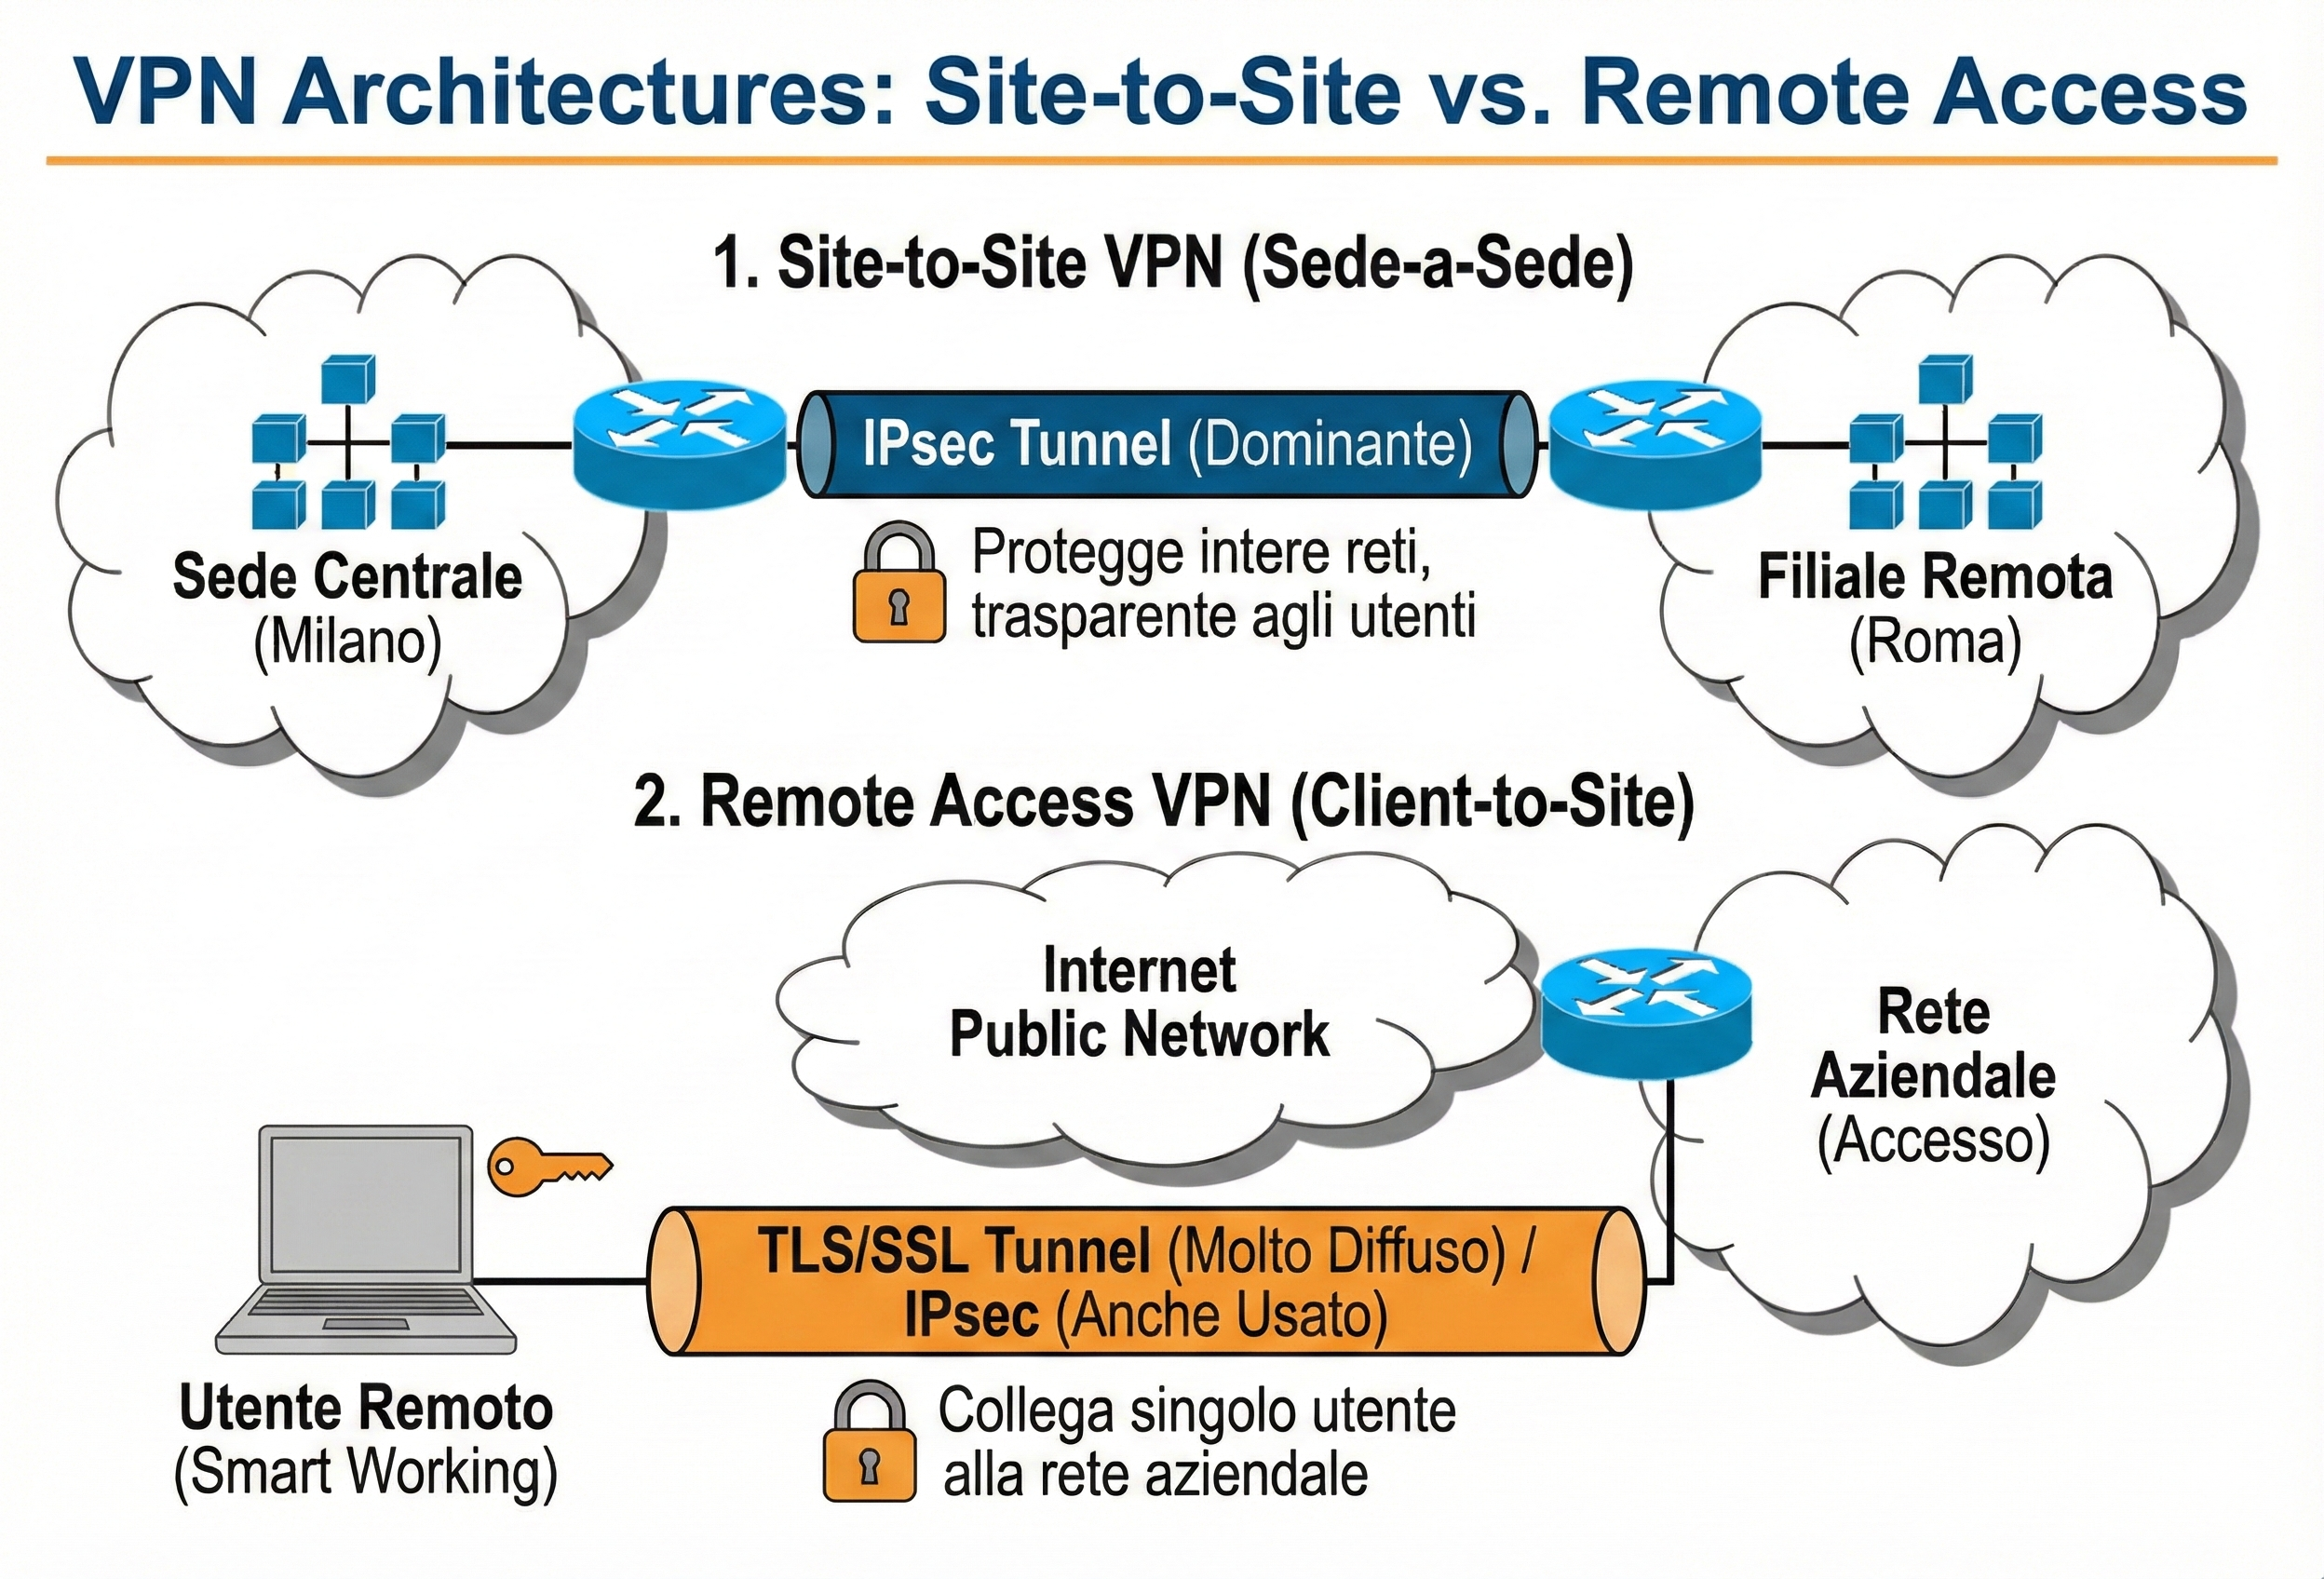
\includegraphics[width=0.8\linewidth]{images/vpn.png}
    \caption{Architettura di esempio di una VPN IPsec (modalità tunnel e transport).}
    \label{fig:vpn}
\end{figure}

Quando si parla di VPN, si ricade quasi sempre in una di queste due architetture (\autoref{fig:vpn}):

\begin{itemize}
    \item \textbf{Site-to-Site}: Collega intere reti (es. la filiale di Roma con la sede di Milano). È trasparente per gli utenti: il router fa tutto il lavoro di cifratura/decifratura. Qui IPsec è il re indiscusso.
    \item \textbf{Remote Access (Client-to-Site)}: Collega un singolo utente (es. in smart working) alla rete aziendale. Qui TLS (SSL) è molto diffuso per praticità, ma si usa anche IPsec.
\end{itemize}

L'utilizzo delle VPN offre molti vantaggi, tra cui:

\begin{enumerate}
    \item \textbf{Riduzione dei Costi}: Prima dell'avvento delle VPN, per collegare una sede di Parigi a Londra in modo sicuro, un'azienda doveva affittare linee fisiche dedicate (Leased Lines), costose e lunghe da installare. Con le VPN, invece, è possibile creare una rete virtuale che collega le due sedi sfruttando l'infrastruttura di Internet già esistente ed economica.
    \item \textbf{Sicurezza}: Poiché Internet è una rete pubblica, è intrinsecamente non sicura. Le VPN permettono di attraversare Internet in sicurezza garantendo i tre pilastri fondamentali: \textbf{confidenzialità, integrità e autenticazione}.
    \item \textbf{Continuità degli Indirizzi IP}: Come visibile nella \autoref{fig:vpn}, una VPN permette di estendere la rete locale privata. Il computer a Roma (es. \texttt{IP 192.168.1.50}) può comunicare con il server a Milano (es. \texttt{IP 192.168.2.10}) come se fossero collegati dallo stesso cavo fisico, rendendo trasparente l'attraversamento della rete pubblica.
    \item \textbf{Scalabilità e Mobilità}: Infine, le VPN offrono grande flessibilità: garantiscono la scalabilità permettendo di collegare facilmente nuove sedi (architettura \textit{site-to-site}) e abilitano la mobilità supportando il lavoro da remoto tramite connessioni sicure per i singoli utenti (architettura \textit{client-to-site}).
\end{enumerate}

Il processo di tunneling (\autoref{fig:vpn_tunnel}) si articola in tre fasi fondamentali:

\begin{enumerate}
    \item \textbf{Fase di Ingresso (Encapsulation)}:
    Tutto ha inizio quando un host nella rete locale (es. \texttt{192.168.1.5}) invia un pacchetto destinato a un host remoto (es. \texttt{10.0.0.2}).
    \begin{itemize}
        \item Il \textbf{Gateway VPN} (o \textit{Tunnel Entry Point}) intercetta questo pacchetto invece di instradarlo normalmente.
        \item Il Gateway considera l'intero pacchetto originale (Header + Dati) come il \textit{payload} di un nuovo pacchetto.
        \item Viene aggiunto un \textbf{Nuovo Header IP} (intestazione esterna). Questo header contiene gli indirizzi IP pubblici necessari per attraversare Internet: l'IP del Gateway mittente come sorgente e l'IP del Gateway destinatario come destinazione.
    \end{itemize}
    \vspace{0.2cm}
    La struttura del pacchetto diventa:
    \[
    \text{Pacchetto Tunneled} = \left[ \underbrace{\text{\textbf{Nuovo Header IP}}}_{\text{IP Pubblici Gateway}} \; \Bigg| \; \underbrace{\text{Header Originale} \; | \; \text{Dati}}_{\text{Payload Incapsulato}} \right]
    \]

    \item \textbf{Fase di Transito}:
    Il pacchetto incapsulato viaggia attraverso l'infrastruttura pubblica (Internet).
    \begin{itemize}
        \item I router intermedi su Internet esaminano esclusivamente il \textbf{Nuovo Header IP} per prendere decisioni di instradamento.
        \item Il contenuto originale è completamente invisibile ("opaco") alla rete di trasporto. I router non sanno che all'interno vi è un altro pacchetto IP, né possono vederne gli indirizzi privati originali.
        \item Dal punto di vista della rete pubblica, sta avvenendo una semplice comunicazione tra due router pubblici (i Gateway VPN).
    \end{itemize}

    \item \textbf{Fase di Uscita (Decapsulation)}:
    Il pacchetto raggiunge il \textbf{Gateway VPN di destinazione} (o \textit{Tunnel Exit Point}).
    \begin{itemize}
        \item Il Gateway analizza l'header esterno e riconosce che si tratta di traffico tunnel destinato a lui.
        \item Procede alla rimozione (\textit{stripping}) del Nuovo Header IP, esponendo nuovamente il pacchetto originale.
        \item A questo punto, il Gateway legge l'Header Originale (che contiene l'IP di destinazione finale, es. \texttt{10.0.0.2}) e instrada il pacchetto nella rete locale interna, esattamente come se fosse arrivato tramite un cavo diretto.
    \end{itemize}
\end{enumerate}

\begin{figure}[ht!]
    \centering
    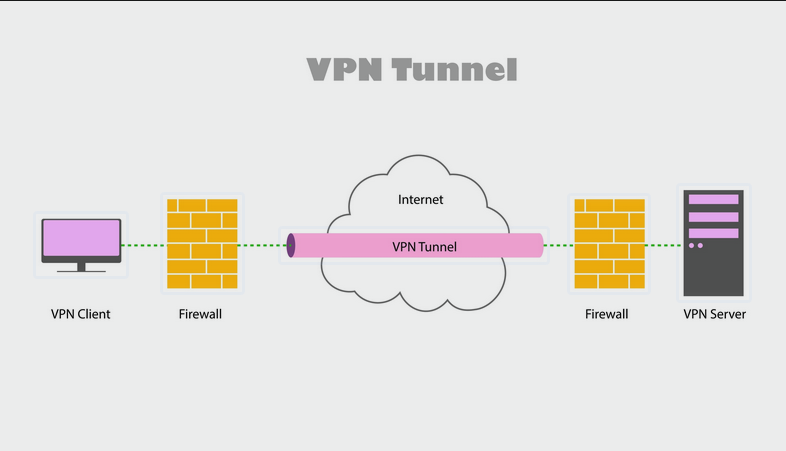
\includegraphics[width=0.8\linewidth]{images/vpn_tunnel.png}
    \caption{VPN Tunneling}
    \label{fig:vpn_tunnel}
\end{figure}

\begin{table}[h!]
    \centering
    \caption{Confronto delle tecnologie VPN e di Tunneling per livello OSI.}
    \label{tab:vpn_layers}
    \renewcommand{\arraystretch}{1.2} % Aumenta leggermente lo spazio tra le righe
    \begin{tabularx}{\textwidth}{@{} l l X @{}}
        \toprule
        \textbf{Livello (Layer)} & \textbf{Tecnologia} & \textbf{Note} \\
        \midrule
        Layer 2 (Data Link) & GRE, PPTP, L2TP & Spesso usati per trasportare traffico non-IP, ma deboli in sicurezza nativa. \\
        \addlinespace
        Layer 3 (Network) & MPLS & Ottimo per performance, nullo per crittografia. \\
        \addlinespace
        Layer 3 (Network) & \textbf{IPsec} & Il \textit{gold standard} per la sicurezza delle reti IP. \\
        \addlinespace
        Layer 4 (Transport) & (D)TLS & Le classiche "SSL VPN" (es. OpenVPN o accesso web sicuro). \\
        \addlinespace
        Layer 7 (App) & SSH Tunnels & Usati spesso dagli amministratori di sistema per accessi rapidi e sicuri. \\
        \bottomrule
    \end{tabularx}
\end{table}

\newpage

\section{IPSec}

IPsec non è un singolo protocollo, ma una suite di protocolli progettata per garantire sicurezza a livello di rete.

A differenza di SSL/TLS che si colloca a metà tra livello di trasporto e applicativo, creando appunto confusione sul utilizzo delle porte, dovendo riservare porte speciali per i protocolli a livello applicativo che usano TLS.
IPsec lavora al Livello 3 (Network Layer) del modello ISO/OSI, e questo comporta differenze architetturali fondamentali:

\begin{itemize}
    \item \textbf{With \& Within IP}: IPsec estende il protocollo IP nativo. I pacchetti IPsec coesistono tranquillamente con pacchetti IP non protetti sulla stessa rete.
    \item \textbf{Trasparenza alle Applicazioni}: Le applicazioni (browser, client email, database) sono inconsapevoli della presenza di IPsec. Non è necessario modificare il software applicativo per usare una VPN IPsec; l'applicazione invia dati normali, e il sistema operativo si occupa di proteggerli prima che lascino la scheda di rete.
    \item \textbf{Protezione "Per-Host"}: La sicurezza è applicata tra host (computer) o tra gateway (router), non tra singole applicazioni o utenti specifici (come invece fa TLS). Quindi IPSec può proteggere tutto il contenuto del pacchetto, non solo l'header.
\end{itemize}

\begin{figure}[ht!]
    \centering
    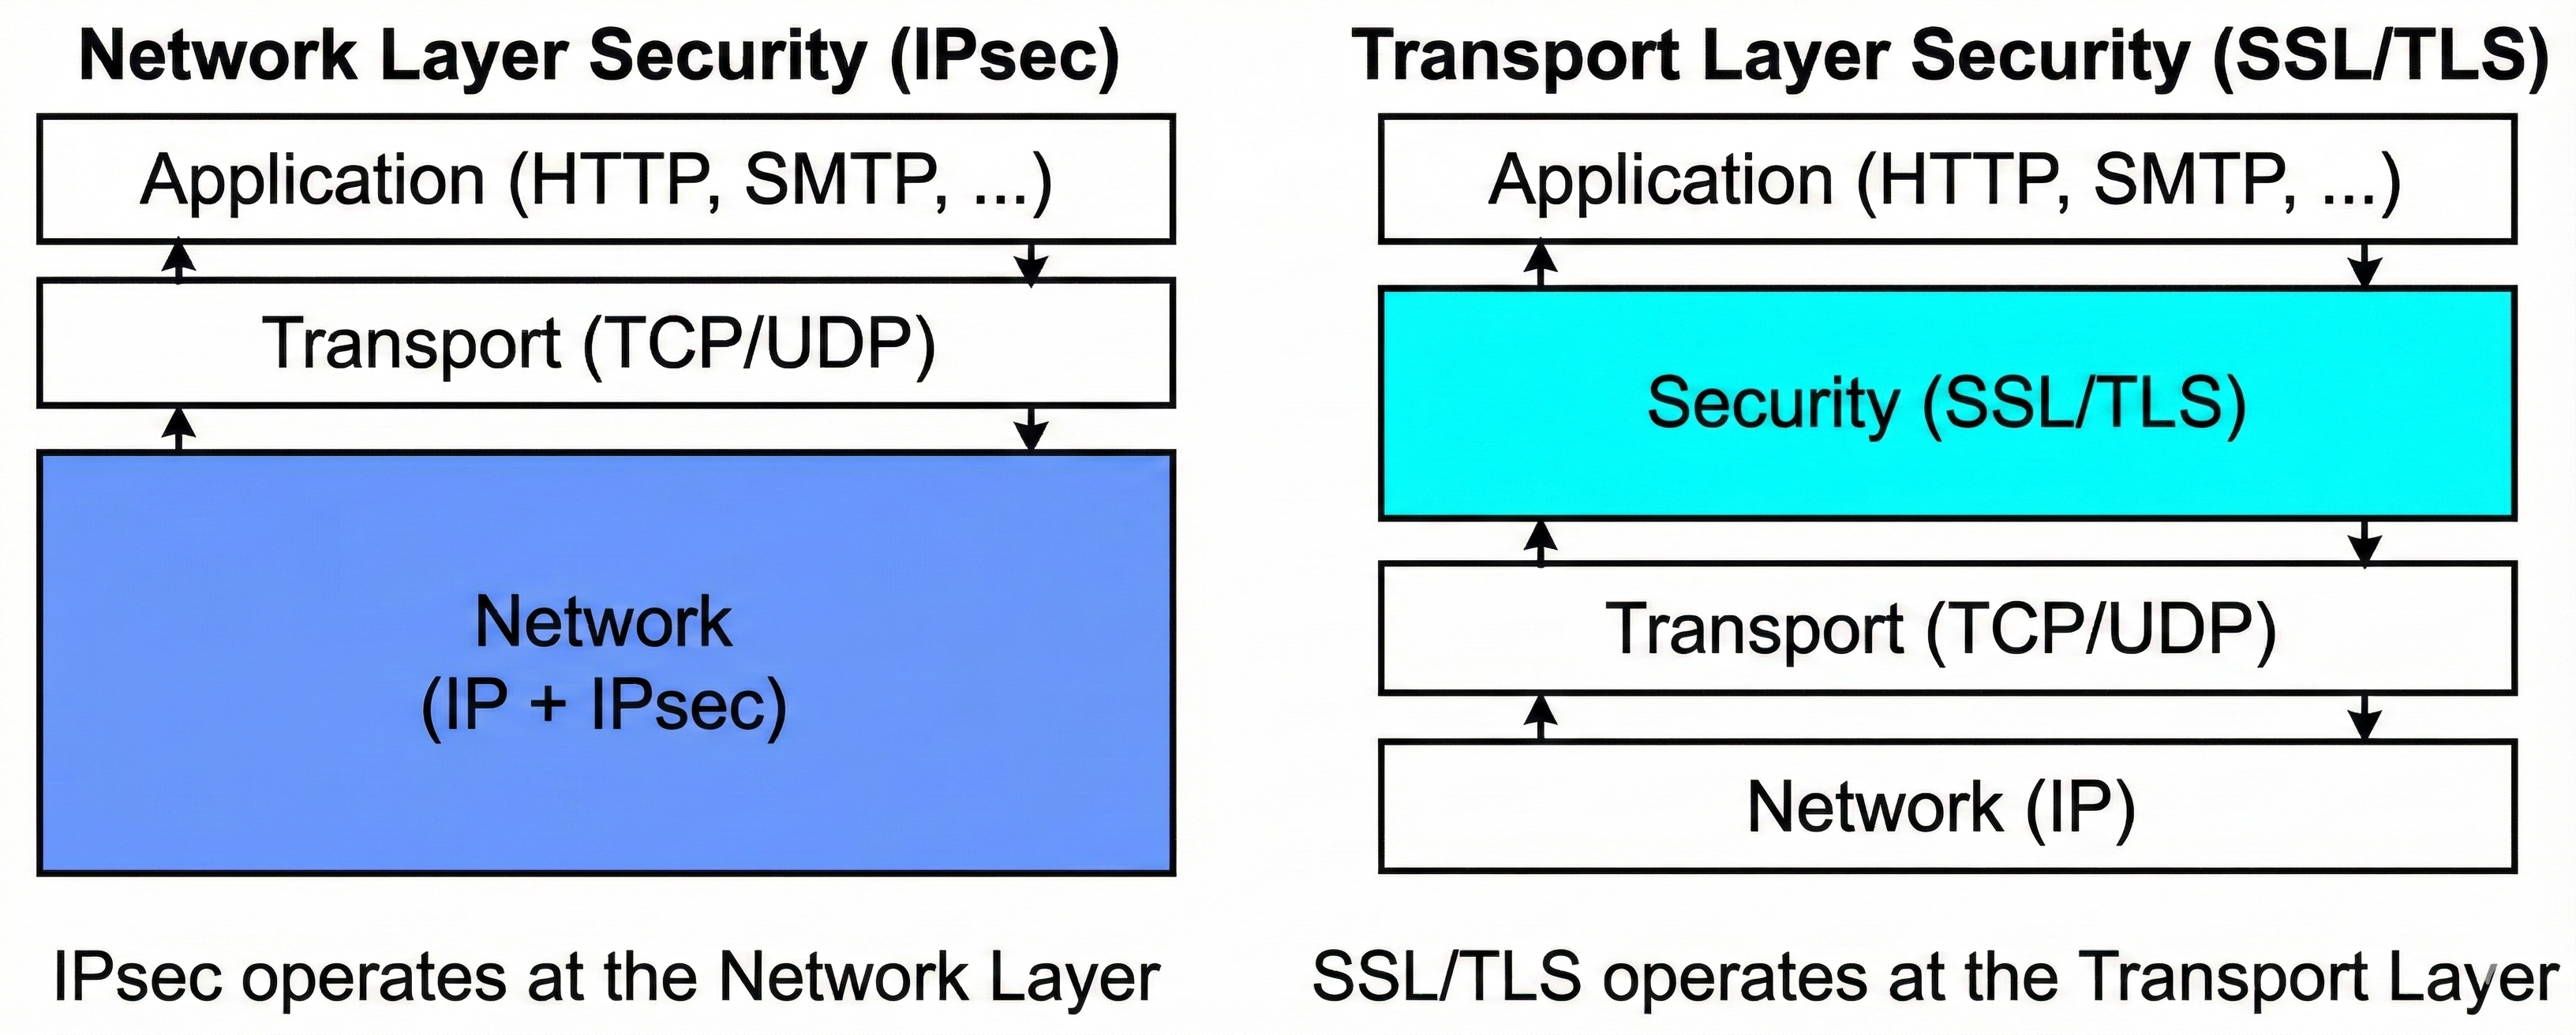
\includegraphics[width=0.8\linewidth]{images/ipsec_tls.png}
    \caption{IPSec vs TLS}
    \label{fig:ipsec_tls}
\end{figure}

Mentre \textbf{TLS (Layer 4)} offre una sicurezza granulare \textit{Process-to-Process}, proteggendo esclusivamente la singola sessione applicativa (socket TCP) e lasciando esposto il resto del traffico della macchina, \textbf{IPsec (Layer 3)} garantisce una protezione \textit{Host-to-Host}. IPsec opera a livello di Kernel e blinda l'intera interfaccia di rete: non discrimina la singola applicazione, ma cifra in blocco tutto il volume di traffico generato da quell'indirizzo IP verso la destinazione, agendo come un tunnel globale e trasparente per qualsiasi protocollo (TCP, UDP, ICMP) transiti per esso.

Poiche non esiste il concetto di sessione, l'architettura IPsec separa strutturalmente la gestione dalla trasmissione, operando su due livelli distinti retti da protocolli dedicati:
\begin{itemize}
    \item \textbf{Il Control Plane (Gestione):} Qui opera il protocollo \textbf{IKE (Internet Key Exchange)}, che ha il compito di negoziare le chiavi e stabilire le \textbf{Security Associations (SA)}, ovvero i "contratti" di sicurezza stabili tra gli host. 
    \item \textbf{Il Data Plane (Traffico):} Una volta attive le SA, intervengono i protocolli \textbf{ESP o AH}, che si limitano ad applicare quelle regole crittografiche per proteggere il flusso di pacchetti IP ad alta velocità. Questa separazione permette, ad esempio, di rinnovare le chiavi (re-keying) tramite IKE senza mai interrompere il flusso dati gestito da ESP.
\end{itemize}

Per fare un esempio banale, prendiamo in considerazione il caso in cui ci colleghiamo ad un access point. Inizialmente avviene una fase di \textbf{handshake (associazione)} in cui si negoziano le chiavi e i parametri di sicurezza. Una volta completata, questo stato di sicurezza (la Security Association) \textit{persiste in memoria} indipendentemente dalla presenza di traffico effettivo. Il canale crittografico rimane "armato" e latente: quando l'host deve trasmettere dati, utilizza immediatamente la configurazione già attiva senza dover rinegoziare i parametri per ogni singolo pacchetto, garantendo efficienza e prontezza.

\subsection{Implementazioni di IPSec}

Sebbene IPsec operi logicamente al \textbf{Livello 3 (Network Layer)} del modello OSI, il codice software effettivo che esegue le operazioni crittografiche può essere collocato in punti differenti della catena di trasmissione. La scelta del punto di inserimento definisce l'architettura di implementazione. Esistono tre approcci principali:

\begin{itemize}
    \item \textbf{Integrated Architecture (Inside Native IP Code)}
    Questo approccio rappresenta lo stato dell'arte per i moderni sistemi operativi (come Linux, Windows 10/11, macOS). In questa configurazione, il supporto a IPsec è \textbf{fuso nativamente} con il codice sorgente del protocollo IP all'interno del Kernel del sistema operativo.
    
    Poiché IPsec e IP sono unificati, non vi è duplicazione di dati o passaggi intermedi: quando il sistema operativo costruisce un pacchetto IP, applica immediatamente le politiche di sicurezza.
    \begin{itemize}
        \item \textbf{Vantaggi}: È l'approccio più efficiente in assoluto. Garantisce le massime performance poiché il codice ha accesso diretto alle strutture dati del kernel senza overhead aggiuntivo.
        \item \textbf{Svantaggi}: La sua implementazione è complessa, in quanto richiede l'accesso e la modifica del codice sorgente del sistema operativo (o l'attesa che il vendor lo implementi).
    \end{itemize}
    \item \textbf{Bump in the Stack (BITS)}
    L'approccio BITS è una tecnica spesso utilizzata per retro-adattare sistemi \textit{Legacy} che non supportano nativamente IPsec (ad esempio, vecchie versioni di Windows).
    Il nome deriva dal fatto che il software di sicurezza viene inserito come uno strato intermedio ("bump") nello stack protocollare, posizionandosi esattamente \textbf{tra l'implementazione nativa di IP e i driver della scheda di rete} (Data Link Layer).
    
    Il funzionamento è trasparente al protocollo IP: il sistema operativo genera un pacchetto in chiaro e lo passa verso il basso; il modulo BITS lo intercetta "al volo", applica la cifratura e solo successivamente lo consegna al driver della scheda di rete per la trasmissione fisica. Oggi questo metodo è raramente utilizzato, essendo IPsec integrato nella maggior parte degli OS moderni.

    \item \textbf{3. Bump in the Wire (BITW)}
    In questo scenario, l'elaborazione crittografica è completamente rimossa dall'host e demandata a un \textbf{dispositivo hardware esterno dedicato} (come un router, un firewall o un concentratore VPN) posizionato fisicamente sulla linea di rete.
    
    Gli host interni alla rete sono totalmente inconsapevoli della presenza di IPsec: essi inviano il traffico in chiaro verso il gateway predefinito. È il dispositivo BITW che intercetta fisicamente il traffico sul cavo, lo cifra e lo instrada su Internet.
    Questa architettura è lo \textbf{standard de facto per le VPN Site-to-Site} aziendali, offrendo vantaggi significativi:
    \begin{itemize}
        \item \textbf{Indipendenza}: Non è necessario installare o configurare alcun software sui computer dei dipendenti.
        \item \textbf{Performance}: Il carico computazionale della crittografia viene scaricato dalle CPU degli host e gestito da processori dedicati sul dispositivo di rete.
    \end{itemize}
\end{itemize}

\subsection{Storia e IPSec Standards}

Lo sviluppo di IPsec è stato un processo iterativo documentato attraverso le \textit{Request for Comments} (RFC) dell'IETF. Possiamo identificare tre fasi storiche principali:

\begin{enumerate}
    \item \textbf{Serie 1 (Agosto 1995) -- RFC 1825-1827}:
    Rappresenta la nascita ufficiale dei concetti di IPsec. Questa prima stesura definiva le basi, ma è oggi considerata obsoleta.

    \item \textbf{Serie 2 (Novembre 1998) -- RFC 2401-2412}:
    Questa fase ha segnato una revisione significativa dell'intera architettura, definendo lo standard IPsec che è stato utilizzato per molti anni (spesso riferito come IPsec v2 o "Legacy IPsec" in alcuni contesti).

    \item \textbf{Serie 3 (Dicembre 2005) -- RFC 4301-4307}:
    È lo standard attuale, nato dopo 5 anni di discussioni nel gruppo di lavoro. Sebbene aggiorni l'intera architettura, l'innovazione cruciale riguarda il protocollo di scambio chiavi:
    \begin{itemize}
        \item Viene introdotto una \textbf{major revision di IKE} (Internet Key Exchange).
        \item Nasce \textbf{IKEv2}, che semplifica drasticamente la gestione unificando e sostituendo i vecchi protocolli separati (ISAKMP, IKEv1, Oakley) in un'unica soluzione più performante.
    \end{itemize}
\end{enumerate}

L'architettura di IPsec (nella sua versione attuale definita dalla \textit{Serie 3}, 2005) è altamente modulare. Non si tratta di un singolo protocollo, ma di una suite di componenti interdipendenti definiti da RFC specifiche:

\begin{itemize}
    \item \textbf{Architettura Generale (The Brain) -- RFC 4301}:
    È il documento fondante che definisce l'architettura di sicurezza e i concetti base, in particolare le \textbf{Security Associations (SA)}. Stabilisce "cosa" deve essere protetto e come gestire il traffico, fungendo da ombrello per tutti gli altri protocolli.

    \item \textbf{Protocolli di Sicurezza (The Muscles) -- Data Plane}:
    Sono i protocolli incaricati di proteggere il traffico dati effettivo.
    \begin{itemize}
        \item \textbf{AH (Authentication Header) - RFC 4302}: Fornisce integrità e autenticazione dell'origine, ma \textit{non} offre confidenzialità (i dati viaggiano in chiaro).
        \item \textbf{ESP (Encapsulating Security Payload) - RFC 4303}: Fornisce confidenzialità (crittografia), autenticazione e integrità. È il protocollo più utilizzato.
        \item \textbf{Algoritmi Crittografici - RFC 4305}: Definisce gli algoritmi specifici (es. AES-GCM, HMAC-SHA) da utilizzare con AH ed ESP.
    \end{itemize}

    \item \textbf{Gestione delle Chiavi (The Negotiator) -- Control Plane}:
    Gestisce l'automazione della sicurezza.
    \begin{itemize}
        \item \textbf{IKEv2 (Internet Key Exchange) - RFC 4306}: Il protocollo per lo scambio automatico delle chiavi e la negoziazione delle SA.
        \item \textbf{Algoritmi per IKEv2 - RFC 4307}: Definisce gli algoritmi crittografici specifici necessari per il funzionamento sicuro di IKE stesso.
    \end{itemize}
\end{itemize}

\newpage

\begin{figure}[ht!]
    \centering
    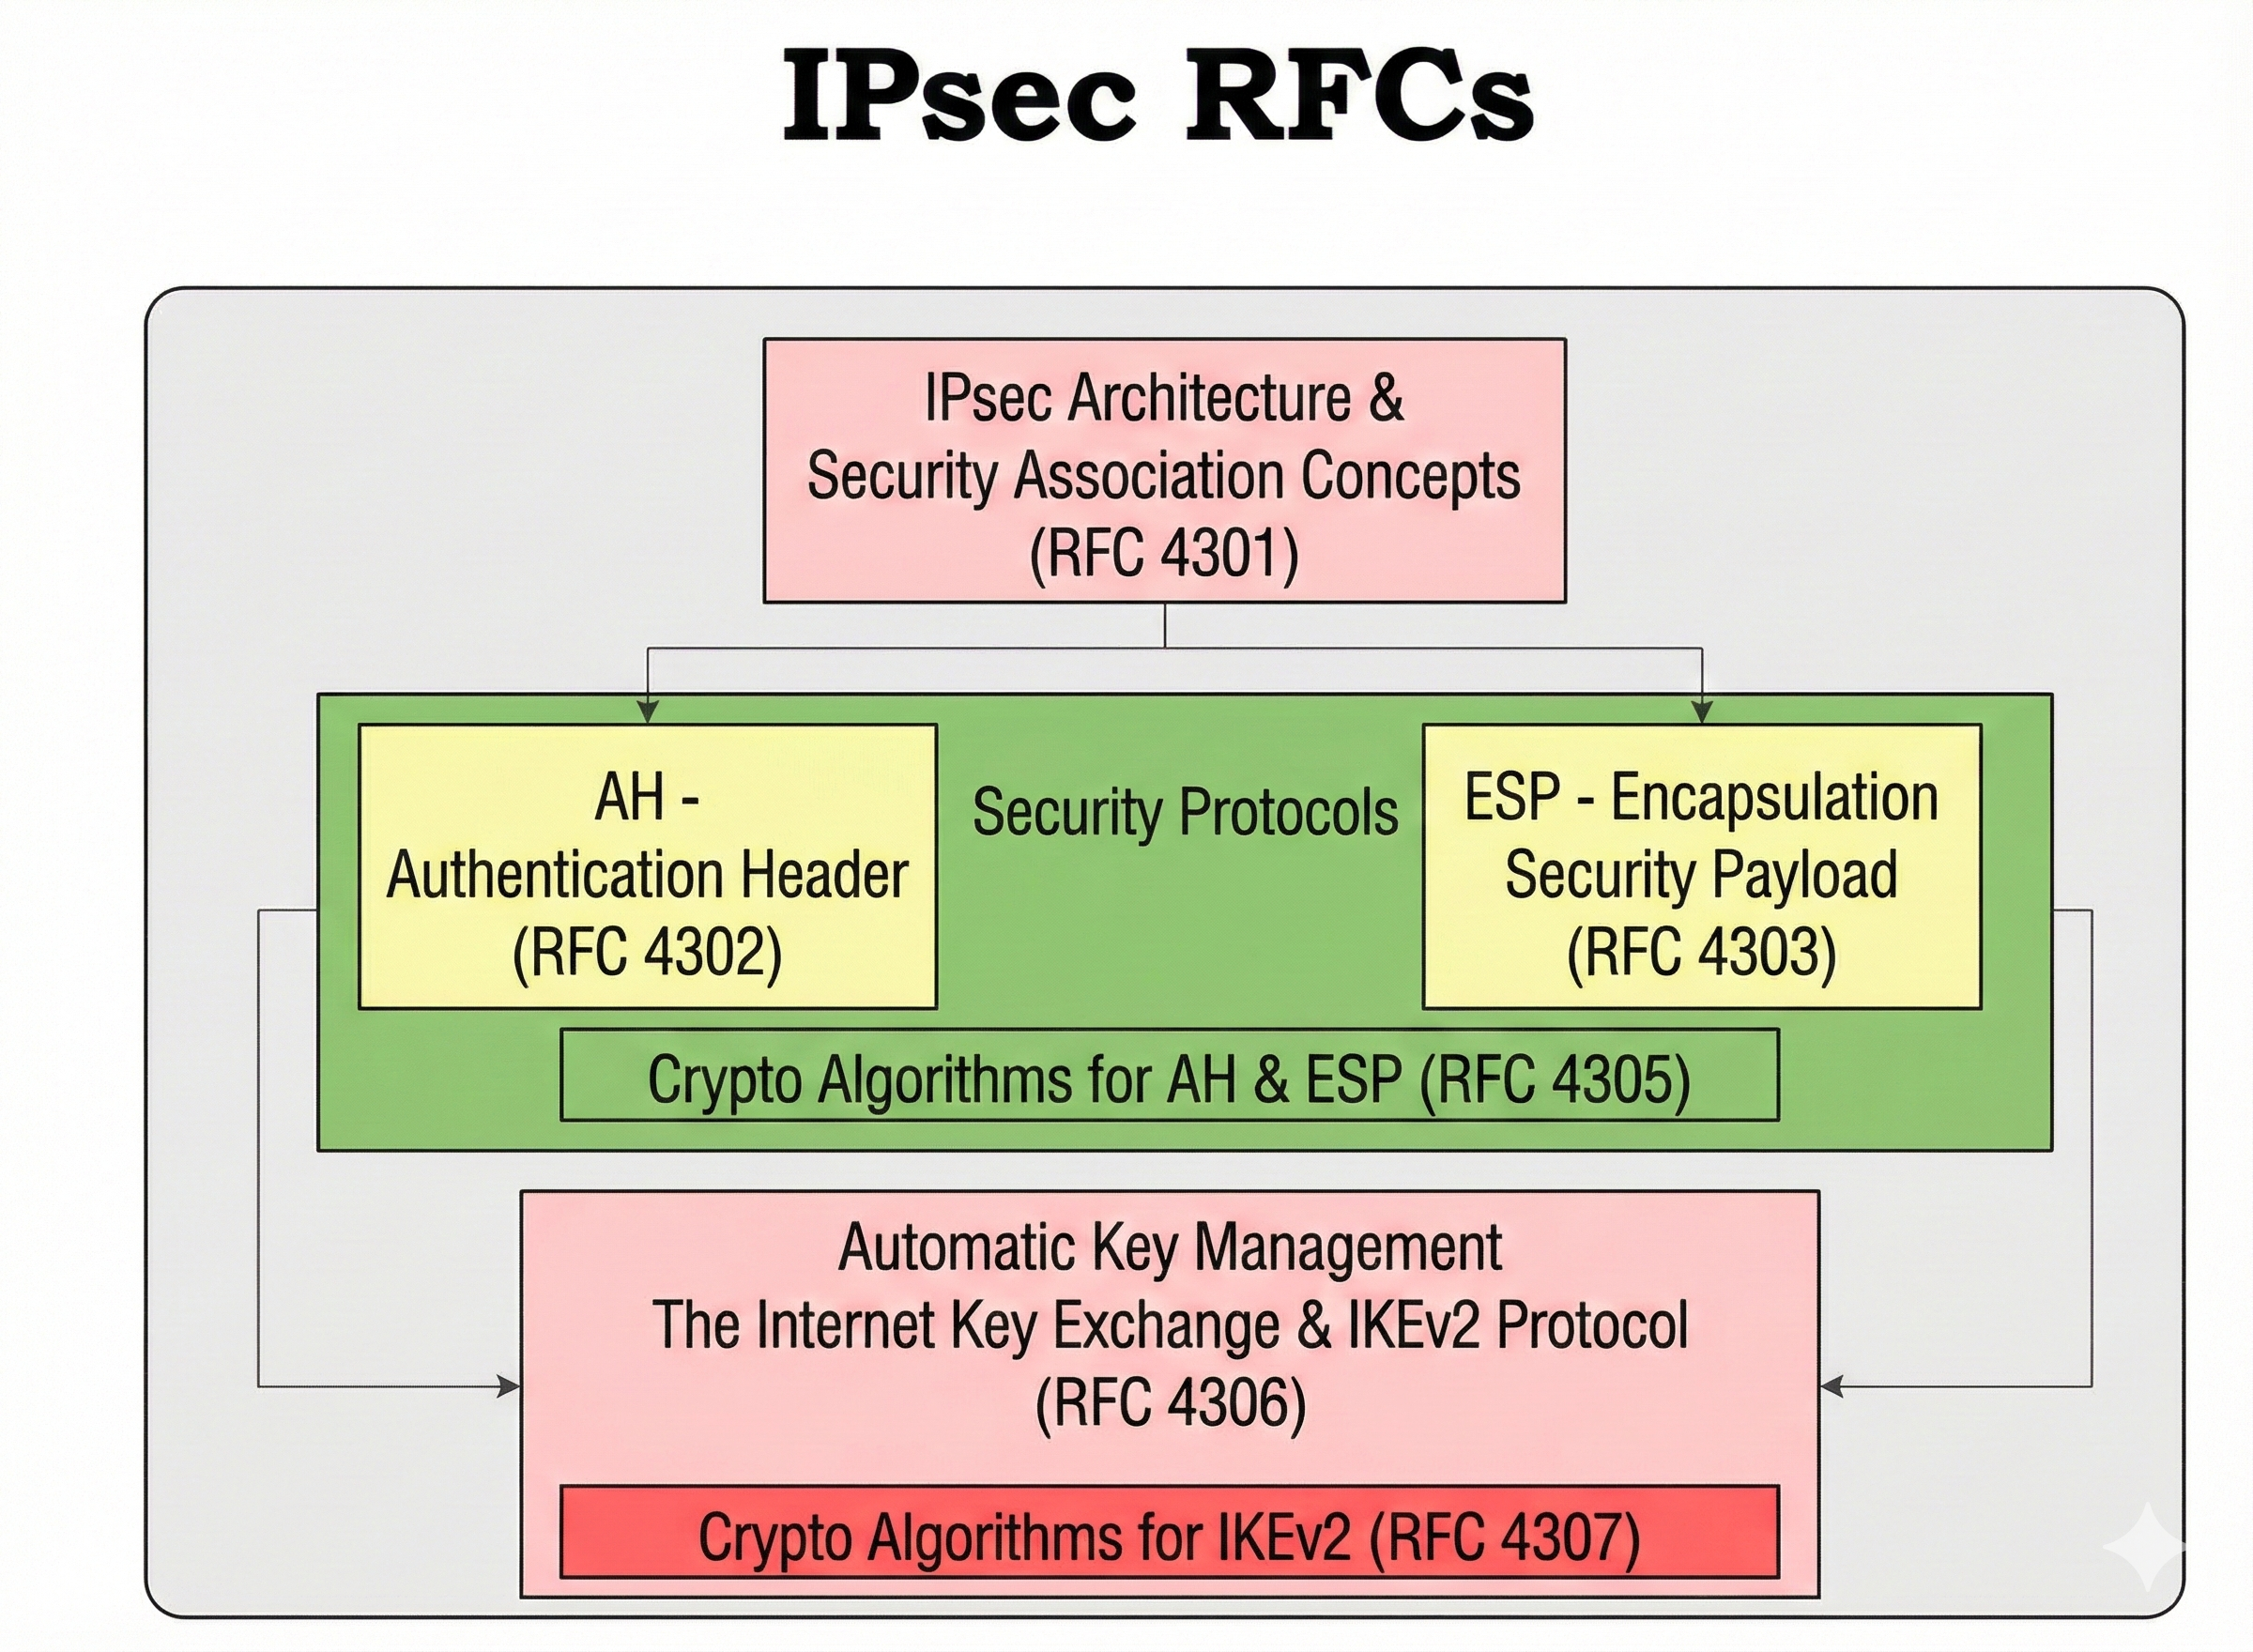
\includegraphics[width=0.6\linewidth]{images/ipsec_protocols.png}
    \caption{Standard IPSec}
    \label{fig:ipsec_protocols}
\end{figure}

\textbf{Nota - Indipendenza Algoritmica}:
Una delle caratteristiche più lungimiranti dell'architettura IPsec è la sua \textbf{Indipendenza Algoritmica} (o \textit{Crypto Agility}).
A differenza di protocolli monolitici, IPsec separa nettamente il \textit{meccanismo di trasporto} (es. il protocollo ESP) dalla \textit{matematica} (l'algoritmo crittografico).

\begin{itemize}
    \item \textbf{Il vantaggio architetturale}: Questa separazione permette di aggiornare la sicurezza nel tempo senza modificare lo stack protocollare. Se un algoritmo diventa obsoleto (es. DES o MD5), è sufficiente aggiornare la configurazione (la \textit{Security Association}) per utilizzare un algoritmo più moderno (es. AES-GCM o SHA-256), mantenendo inalterato il protocollo ESP.

    \item \textbf{Confronto con TLS Legacy}: Questo approccio contrasta con le versioni iniziali di altri protocolli di sicurezza, come SSL/TLS.
    \begin{quote}
    \textit{Esempio:} In \textbf{TLS 1.1}, primitive critiche come la \textbf{PRF} (Pseudo-Random Function) erano \textit{hard-coded} (basate su MD5/SHA-1). Non era possibile negoziarle: per cambiare la funzione di derivazione delle chiavi, era necessario aggiornare l'intera versione del protocollo a TLS 1.2 (che ha introdotto la negoziabilità della PRF).
    \end{quote}
    IPsec, al contrario, ha sempre trattato gli algoritmi come "plugin" intercambiabili, garantendo una maggiore longevità dell'infrastruttura di rete.
\end{itemize}

\section{Security Association}

A differenza di protocolli come TLS, che proteggono una specifica connessione "session-oriented", IPsec introduce il concetto fondamentale di \textbf{Security Association (SA)}.
La SA non rappresenta una connessione attiva, bensì un \textbf{accordo logico} tra due entità sui parametri di sicurezza da applicare ai pacchetti.

Le Security Associations in IPsec sono flessibili e possono essere stabilite tra diverse tipologie di endpoint. Si distinguono tre scenari principali di dispiegamento:

\begin{enumerate}
    \item \textbf{Host-to-Host (End-to-End Security)}:
    In questo scenario la SA viene negoziata direttamente fra due singoli host — per esempio due server o un client e un server — e la protezione si estende dall'interfaccia di rete del mittente fino a quella del destinatario. I pacchetti non lasciano mai la rete in chiaro: header e payload sono protetti end-to-end, tipicamente nella modalità \textit{transport}, fornendo il massimo livello di riservatezza e integrità per le comunicazioni punto-a-punto.

    \item \textbf{Host-to-Gateway (Remote Access VPN)}:
    Qui la SA è stabilita tra un singolo host (ad esempio il portatile di un utente remoto) e un gateway aziendale. L'host incapsula il proprio traffico e lo invia attraverso un tunnel verso il gateway, che provvede a decapsularlo e a inserirlo nella rete interna. Questo modello, comune per l'accesso remoto, fa sì che l'utente remoto venga trattato come se fosse connesso localmente alla LAN; per proteggere gli indirizzi e l'intera sottorete si utilizza solitamente la \textit{tunnel mode}.

    \item \textbf{Gateway-to-Gateway (Site-to-Site VPN)}:
    In questo caso la SA viene negoziata tra due dispositivi di rete (router, firewall o concentratori VPN) che proteggono intere reti locali. Gli host interni inviano il traffico in chiaro fino al proprio gateway, il quale si occupa di cifrarlo prima di trasmetterlo sulla rete pubblica: all'altro capo, il gateway destinatario decifra e reimmette i pacchetti nella LAN remota. Questa architettura è tipica delle VPN fra sedi e richiede generalmente la \textit{tunnel mode} per garantire la protezione degli indirizzi interni.
\end{enumerate}

Le caratteristiche distintive della SA sono:
\begin{itemize}
    \item \textbf{Unidirezionale}:
    La natura \textit{simplex} (unidirezionale) delle Security Associations non è un limite, ma una scelta architetturale che garantisce grande granularità.
    Per proteggere una comunicazione bidirezionale sono necessarie due SA distinte (una \textit{Inbound} e una \textit{Outbound}).
    Questo disaccoppiamento permette di implementare \textbf{politiche di sicurezza asimmetriche}:
    \begin{itemize}
        \item È possibile utilizzare algoritmi crittografici differenti per l'andata e per il ritorno (es. cifratura pesante in una direzione e leggera nell'altra).
        \item È possibile applicare protocolli diversi (es. ESP per confidenzialità in uscita, AH per sola integrità in entrata), ottimizzando il carico computazionale in base alla sensibilità reale dei dati in ciascuna direzione.
    \end{itemize}

    \item \textbf{Contratto di Parametri}:
    La SA è una struttura dati complessa che definisce in dettaglio "come" proteggere i dati. Oltre agli algoritmi di base, include parametri di stato critici per la sicurezza operativa:
    \begin{itemize}
        \item \textbf{Primitive Crittografiche}: Specifica l'algoritmo di cifratura (es. AES-CBC, AES-GCM) e l'algoritmo di integrità (es. HMAC-SHA256), con le relative chiavi segrete operative.
        \item \textbf{Sequence Number Counter}: Un contatore incrementale (a 32 o 64 bit) per i pacchetti in uscita. Questo numero viene inserito in ogni pacchetto e serve a garantire l'unicità e l'ordine, prevenendo attacchi di tipo \textit{Replay}.
        \item \textbf{Anti-Replay Window}: Una finestra scorrevole (bitmask) utilizzata dal ricevente per tracciare i numeri di sequenza già validati e scartare duplicati o pacchetti malevoli "vecchi" reinseriti nella rete da un attaccante.
        \item \textbf{Lifetime (Soft \& Hard Limits)}: La scadenza della SA non è basata solo sul \textbf{tempo} (es. 3600 secondi), ma anche sul \textbf{volume di dati} (es. 100 MB). Questo impedisce a un attaccante di raccogliere troppi campioni cifrati con la stessa chiave, forzando un rinnovo frequente (Re-keying).
        \item \textbf{IPsec Mode}: L'indicazione se la SA deve operare in modalità \textit{Tunnel} o \textit{Transport}.
    \end{itemize}

    \item \textbf{Identificazione tramite SPI}:
    Poiché su una singola interfaccia di rete possono coesistere molteplici SA unidirezionali e indipendenti, è indispensabile un meccanismo di disambiguazione per associare ogni pacchetto al corretto "contratto" di sicurezza.
    
    Questo ruolo è svolto dallo \textbf{SPI (Security Parameter Index)}: un'etichetta numerica univoca a 32 bit inserita nell'header del pacchetto (ESP o AH). Il ricevente utilizza la tripla 
    \[
        \langle\texttt{SPI,\ IP Destinazione,\ Protocollo (ESP/AH)}\rangle
    \]
    come chiave di ricerca per interrogare il \textbf{SAD (Security Association Database)}, recuperare la SA specifica e decifrare correttamente il flusso dati.

    \textbf{Perché l'IP non basta come identficativo?}
    L'indirizzo IP non è sufficiente per identificare univocamente una Security Association (SA) poiché la relazione tra Host e SA è di tipo \textbf{uno-a-molti}.
    L'utilizzo dell'SPI (Security Parameter Index) è necessario per gestire situazioni in cui esistono più canali sicuri tra gli stessi due IP:
    \begin{itemize}
        \item \textbf{Differenziazione dei servizi}: Permette di applicare politiche di sicurezza diverse a flussi diversi provenienti dallo stesso host (es. una SA ad alta cifratura per transazioni critiche e una SA a bassa latenza per VoIP).
        \item \textbf{Gestione del Re-keying}: Durante il rinnovo delle chiavi, la "vecchia SA" e la "nuova SA" si sovrappongono temporalmente. L'SPI permette al ricevente di distinguere quale chiave utilizzare per decifrare lo specifico pacchetto in arrivo.
    \end{itemize}
\end{itemize}

La creazione e la gestione delle Security Associations (SA) può avvenire secondo due modalità principali: configurazione manuale o negoziazione automatica.

\begin{enumerate}
    \item \textbf{Gestione Manuale (Manual Keying)}:
    È un metodo essenziale in cui l'amministratore configura staticamente le chiavi su ogni dispositivo. Sebbene sia funzionale per collegamenti semplici e stabili (es. tra due sole sedi), diventa rapidamente ingestibile al crescere della rete: in topologie complesse il numero di configurazioni esplode (problema di scalabilità $N^2$) e l'assenza di rinnovo automatico delle chiavi espone il sistema a gravi rischi di sicurezza nel lungo periodo.

    \item \textbf{Gestione Automatica (Automatic Keying)}:
    Rappresenta lo standard moderno, affidato al protocollo \textbf{IKEv2}. Questo approccio crea le SA dinamicamente e "on-demand" solo quando c'è traffico, ottimizzando le risorse. Grazie al rinnovo automatico e frequente delle chiavi (\textit{rekeying}), garantisce livelli di sicurezza superiori (come la Perfect Forward Secrecy) e permette di gestire grandi infrastrutture in modo flessibile e scalabile, riducendo drasticamente l'errore umano.
\end{enumerate}

\newpage

\section{IPSec Security Protocols}

Il framework IPsec si basa su due protocolli principali per fornire sicurezza al traffico IP: \textbf{AH} (Authentication Header) ed \textbf{ESP} (Encapsulating Security Payload). Entrambi possono operare sia in modalità \textit{Transport} che in modalità \textit{Tunnel}.

\subsection{Authentication Header}

Il protocollo AH è progettato per garantire l'autenticità e l'integrità, ma \textbf{non offre confidenzialità} (non cifra i dati).

IPsec Authentication Header (AH) è nato per fornire garanzie di integrità e autenticazione dell'origine dei pacchetti IP, ma non per garantire la confidenzialità: i dati non vengono cifrati. In pratica, AH calcola un valore di autenticazione (un MAC/HMAC) che copre gran parte del pacchetto IP, consentendo al destinatario di verificare che il pacchetto provenga effettivamente dal mittente dichiarato e che non sia stato alterato durante il transito.

Una caratteristica distintiva di AH è proprio la sua ampia copertura: oltre al payload, AH autentica anche gran parte dell'header IP originale, fatta eccezione per i campi \textit{mutabili} che possono cambiare legittimamente durante l'instradamento (ad esempio il TTL o certi campi modificati da dispositivi intermedi). Questo comportamento rende AH utile quando è richiesta l'autenticazione dell'header stesso, ma lo rende anche vulnerabile a scenari in cui i dispositivi intermedi modificano gli header (come nel caso del NAT), nei quali AH risulta spesso incompatibile.

AH offre inoltre protezione contro gli attacchi di replay tramite l'uso di numeri di sequenza e di finestre anti-replay; è possibile anche l'uso di Extended Sequence Numbers per scenari ad alto throughput. Nonostante ciò, nella pratica moderna AH è ormai meno diffuso: la maggior parte delle implementazioni preferisce ESP, che può fornire sia confidenzialità che autenticazione del payload (e, se necessario, comportamenti comparabili ad AH). Per questo motivo la RFC 4301 ha ridotto il vincolo sul supporto di AH da obbligatorio a facoltativo (da MUST a MAY), lasciando AH come soluzione utile in casi particolari ma non come elemento imprescindibile dell'ecosistema IPsec.

\begin{figure}[ht!]
    \centering
    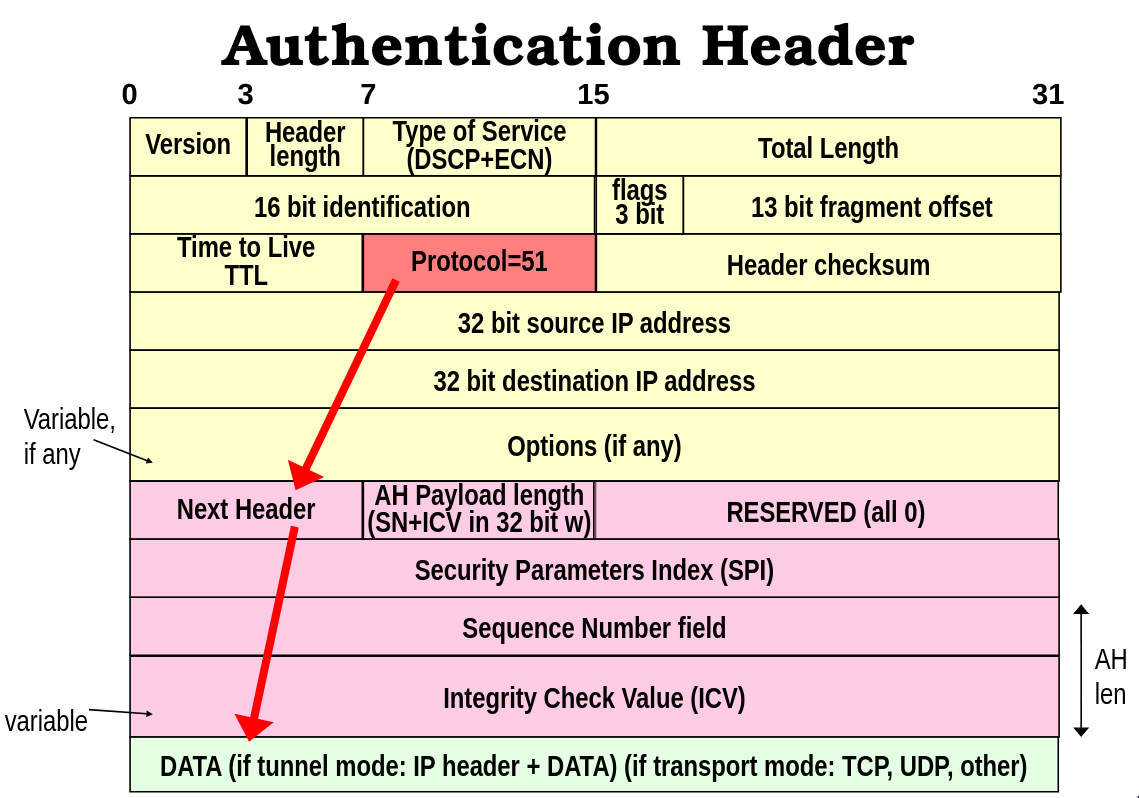
\includegraphics[width=0.8\linewidth]{images/ah_header.png}
    \caption{Authentication Header insime al Pacchetto IP}
    \label{fig:ah_header}
\end{figure}

Un vantaggio architetturale significativo di IPsec rispetto a TLS risiede nella gestione dell'incapsulamento e nell'identificazione dei protocolli.

Un limite pratico di TLS deriva dalla sua collocazione sopra il livello di trasporto: per offrire versioni sicure di protocolli applicativi si tende spesso a usare porte TCP dedicate (ad esempio HTTP 80 $\to$ HTTPS 443, LDAP 389 $\to$ LDAPS 636) oppure meccanismi come STARTTLS. Questo comportamento comporta una duplicazione delle porte conosciute e introduce complessità operative nella gestione di firewall, NAT e policy di rete, soprattutto in scenari con molteplici servizi e vincoli di instradamento.

IPsec, invece, si inserisce nello stack in modo più "pulito" e trasparente. Come mostrato in \autoref{fig:ah_header}, la presenza di IPsec è segnalata dall'header IP esterno tramite il campo \texttt{Protocol} (valori tipici: 51 per AH, 50 per ESP). All'interno dell'header AH o ESP è presente il campo \texttt{Next Header}, che indica quale protocollo è incapsulato (ad esempio TCP, UDP o — in modalità tunnel — un altro pacchetto IP). Grazie a questo meccanismo non è necessario ridefinire porte applicative: le applicazioni mantengono le loro porte originali e il traffico viene semplicemente trasportato all'interno della "busta" IPsec. Questo approccio evita l'"esplosione" delle porte e rende l'incapsulamento strutturalmente più corretto e facilmente scalabile nella gestione delle reti sicure.

Altri campi dell'AH:
\begin{itemize}
    \item \texttt{Security Parameters Index (SPI)}: usato per ricavare dal database i parametri crittografici.
    \item \texttt{Sequence Number Field}: Un numero di sequenza (32 bit) monotono strettamente crescente (incrementato di 1 per ogni pacchetto inviato) per prevenire attacchi di replay.
    \item \texttt{Integrity Check Value (ICV)}: è tipicamente calcolato tramite un HMAC (o altra funzione di autenticazione) per verificare integrità e autenticità del pacchetto. Nel caso di AH l'ICV copre gran parte dell'header IP originale (escludendo o normalizzando i campi mutabili) e i campi dell'header AH stesso. 
\end{itemize}

\subsubsection{Servizio Anti-Replay e Sequence Numbers}

Uno dei servizi opzionali (ma raccomandati e attivi di default) di IPsec è la protezione contro i \textbf{Replay Attacks}. Poiché l'header IP nativo non possiede un numero di sequenza, un attaccante potrebbe intercettare un pacchetto cifrato valido e ritrasmetterlo successivamente per duplicare l'azione (es. duplicare una transazione bancaria).

Per mitigare questo rischio, IPsec introduce un campo \textbf{Sequence Number} nell'header (AH o ESP). È un contatore incrementale di 32 bit gestito come segue:

\begin{itemize}
    \item \textbf{Inizializzazione}: Al momento della creazione della Security Association (SA), il contatore viene impostato a 0.
    \item \textbf{Incremento}: Il primo pacchetto trasmesso avrà $SN=1$. Il contatore viene incrementato di 1 per ogni pacchetto successivo.
    \item \textbf{Verifica}: Il ricevente mantiene una "finestra scorrevole" (\textit{sliding window}) per scartare pacchetti con numeri vecchi (già ricevuti) o troppo fuori sequenza.
\end{itemize}

Una regola ferrea di IPsec è che il Sequence Number \textbf{non può mai ricominciare da zero (wrap-around)}.

\begin{quote}
    \textit{Limite Operativo}: Una volta raggiunto il valore massimo ($2^{32}-1$, circa 4.3 miliardi di pacchetti), la SA corrente \textbf{deve essere terminata} immediatamente e ne deve essere negoziata una nuova (con nuove chiavi).
\end{quote}

Questo vincolo è necessario per preservare la sicurezza crittografica: riutilizzare lo stesso contatore con la stessa chiave crittografica comprometterebbe l'unicità del \textit{Keystream} (specialmente in modalità come CTR o GCM), rendendo banale la decifrazione del traffico.

\paragraph{Extended Sequence Number (ESN)}
Con l'aumento delle velocità di rete, il limite dei 32 bit è diventato un collo di bottiglia. A 1 Gbps con MTU 1500 si esaurisce in $\sim$14 ore, mentre a 10-40 Gbps la SA potrebbe scadere in pochi minuti. 
La RFC 4303 risolve il problema introducendo l'\textbf{Extended Sequence Number a 64 bit}, ma senza aumentare l'overhead sul filo: viene trasmessa solo la parte bassa (low-order 32 bit) mentre i 32 bit alti sono mantenuti e sincronizzati localmente. Per preservare la sicurezza, il valore completo a 64 bit è incluso nel calcolo dell'ICV.

\subsubsection{Meccanismo della Sliding Window (Anti-Replay)}

Per difendersi dai replay attack IPsec adotta una finestra scorrevole di dimensione W gestita dal ricevente. La dimensione non è negoziata (tipicamente minima 32, default 64) e il margine destro della finestra coincide con il Sequence Number più alto già accettato.

Il comportamento è semplice e robusto: quando arriva un pacchetto con numero di sequenza SeqN il ricevente procede così — se SeqN è troppo piccolo (a sinistra della finestra) il pacchetto viene scartato; se SeqN cade nella finestra si verifica la bitmask per rilevare duplicati e si controlla l'ICV: se l'ICV è valido il pacchetto viene accettato e il corrispondente bit viene marcato; se SeqN è maggiore del margine destro il pacchetto è nuovo e, dopo aver validato l'ICV, la finestra viene fatta scorrere a destra aggiornando il nuovo margine e scartando i bit ormai fuori range.

Regole operative importanti: non si sposta la finestra prima della verifica dell'ICV (evitando facili DoS) e lo Sequence Number non deve mai riavvolgersi (wrap-around), pena la terminazione della SA e la negoziazione di una nuova.

\subsection{Encapsulated Security Payload}

ESP è il protocollo più completo e flessibile, oggi considerato lo standard \textit{de facto} per la maggior parte delle implementazioni IPsec.

ESP (Encapsulating Security Payload) è il protocollo più utilizzato nella suite IPsec perché fornisce un insieme completo di servizi di protezione per il traffico IP. La sua caratteristica principale è la capacità di garantire la confidenzialità dei dati: il payload dei pacchetti viene cifrato con algoritmi di crittografia moderni in modo che il contenuto rimanga illeggibile a chi intercetti il traffico. Oltre alla cifratura, ESP può anche fornire autenticazione e integrità del payload, consentendo al destinatario di verificare che i dati non siano stati alterati durante il transito e che provengano dalla fonte attesa.

ESP riduce le informazioni visibili: campi come \texttt{Next Header} e \texttt{Pad Length} sono nel trailer cifrato, e padding o traffico fittizio possono mitigare la \textbf{traffic analysis}. Supporta primitive AEAD (es. AES-GCM) che combinano cifratura e autenticazione in modo efficiente.

I campi \texttt{SPI} e \texttt{Sequence Number} restano in chiaro, mentre il payload e il trailer vengono cifrati.

ESP è oggi lo standard pratico per IPsec: offre confidenzialità, integrità e autenticazione ed è richiesto dalla maggior parte delle implementazioni moderne. Può essere configurato con "null encryption" per fornire solo integrità (comportamento simile ad AH) ma con maggiore flessibilità e compatibilità (es. in presenza di NAT).

\begin{figure}[ht!]
    \centering
    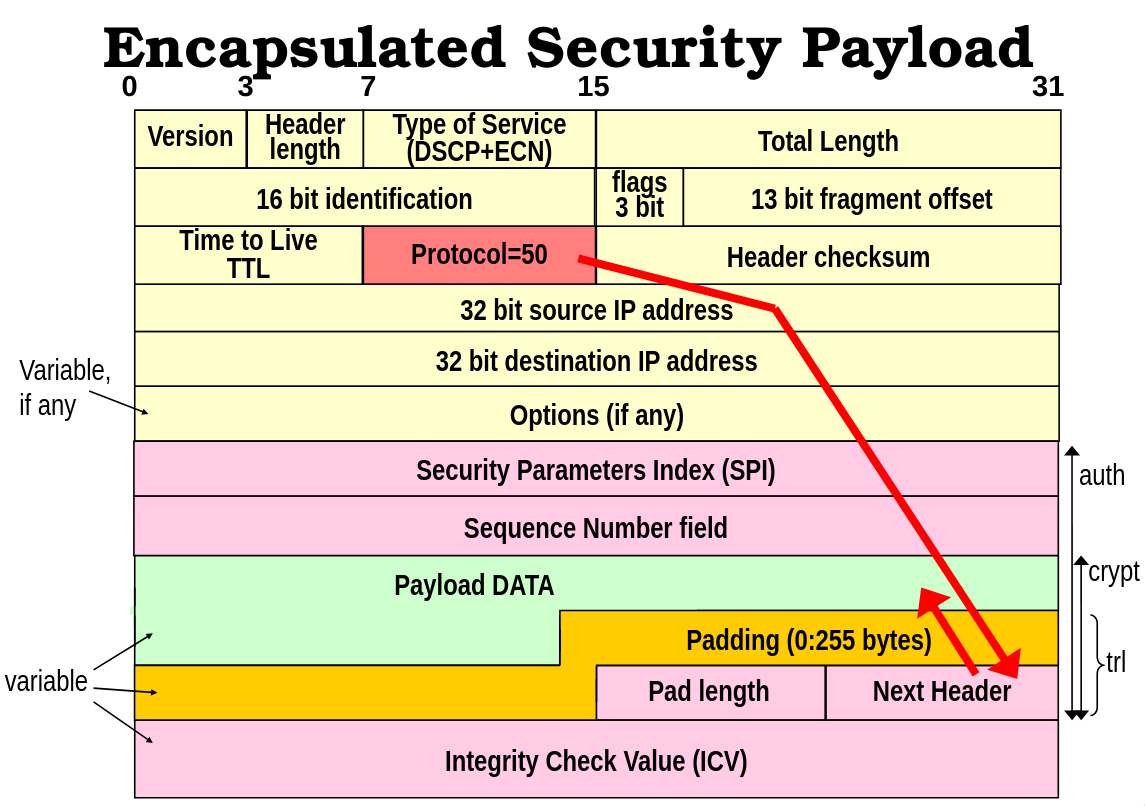
\includegraphics[width=0.6\linewidth]{images/esp.png}
    \caption{ESP insime insieme al Pacchetto IP}
    \label{fig:esp}
\end{figure}

\newpage

\subsection{Modalità Operative: Transport vs Tunnel}

Entrambi i protocolli possono funzionare in due modalità architettoniche distinte, che modificano radicalmente la struttura del pacchetto.

\subsubsection{Transport Mode}
Utilizzata tipicamente per comunicazioni \textit{Host-to-Host}. Mantiene l'header IP originale.
In modalità transport l'obiettivo è proteggere il contenuto della comunicazione mantenendo inalterato l'header IP originale: questa scelta è tipica delle comunicazioni Host-to-Host, dove si vuole salvaguardare i dati scambiati tra due endpoint senza incapsulare l'intero pacchetto. A seconda del protocollo scelto (AH o ESP) cambia però la semantica precisa della protezione.

\textbf{Con AH}: l'header AH viene inserito immediatamente dopo l'header IP originale e prima del payload (TCP/UDP). AH calcola un valore di autenticazione che copre gran parte del pacchetto, inclusi molti campi dell'header IP (esclusi quelli mutabili come TTL); questo permette di verificare autenticità e integrità sia dell'header sia del payload. Tale comportamento rende AH poco compatibile con dispositivi che modificano gli header in transito (ad es. NAT). 
\[
    [\text{IP Header}] \; [\textbf{AH}] \; [\text{TCP/UDP}] \; [\text{Data}]
\]
\textbf{Con ESP}: l'header ESP è inserito subito dopo l'header IP; a differenza di AH, ESP può cifrare il payload (TCP/UDP + dati) lasciando l'header IP in chiaro per l'instradamento. L'autenticazione con ESP copre l'header ESP e i campi fino al trailer, ma non l'header IP esterno; quando si usano primitive AEAD (es. AES-GCM) cifratura e autenticazione sono combinate in modo efficiente. Questa modalità è generalmente più pratica in presenza di NAT e più diffusa nelle implementazioni reali.
\[
    [\text{IP Header}] \; [\textbf{ESP Hdr}] \; \underbrace{[\text{TCP/UDP}] \; [\text{Data}]}_{\text{Cifrati}} \; [\text{ESP Trl}] \; [\text{ESP Auth}]
\]

\subsubsection{Tunnel Mode}
Utilizzata tipicamente per VPN \textit{Site-to-Site} (Gateway-to-Gateway). Il pacchetto originale viene incapsulato dentro un nuovo pacchetto.
In modalità tunnel, l'intero pacchetto originale — comprensivo dell'header IP interno — viene trattato come payload e viene incapsulato all'interno di un nuovo pacchetto con un nuovo header IP esterno. Questa scelta è tipica delle VPN site-to-site, dove si vuole nascondere sia i dati che gli indirizzi interni alla rete privata.

\textbf{Con AH:} in tunnel mode l'header AH viene inserito tra il nuovo header IP esterno e il pacchetto originale incapsulato. AH fornisce autenticazione e integrità su una porzione ampia del pacchetto: nel caso di tunnel autentica il nuovo header IP (nel limite dei campi non mutabili), l'header AH e l'intero pacchetto originale che è stato incapsulato. In pratica, il ricevente verifica che il pacchetto non sia stato alterato e che provenga dalla fonte attesa prima di rimuovere l'incapsulamento e reinoltrare il pacchetto interno nella LAN. Una rappresentazione sintetica della struttura è:
\[
    [\text{\textbf{New IP}}] \; [\textbf{AH}] \; [\text{Orig IP}] \; [\text{TCP/UDP}] \; [\text{Data}]
\]

\textbf{Con ESP:} in tunnel mode ESP cifra e (se configurato) autentica l'intero pacchetto originale, inclusivo dell'header IP interno. Sulla rete pubblica resta quindi visibile solo il nuovo header IP esterno, necessario per l'instradamento tra gateway, mentre il contenuto interno è protetto dalla crittografia. L'autenticazione copre i campi dall'header ESP fino al trailer; va però tenuto presente che il nuovo header IP esterno non è protetto da ESP, per cui qualsiasi modifica a quel livello va gestita a parte. La struttura tipica è:
\[
    [\text{\textbf{New IP}}] \; [\textbf{ESP Hdr}] \; \underbrace{[\text{Orig IP}] \; [\text{TCP/UDP}] \; [\text{Data}]}_{\text{Cifrati}} \; [\text{ESP Trl}] \; [\text{ESP Auth}]
\]

In conlusione, AH in tunnel fornisce soprattutto integrità e autenticazione anche dell'incapsulamento, mentre ESP in tunnel è la scelta più comune quando si desidera riservatezza completa del traffico interno, abbinabile opzionalmente all'autenticazione per garantire anche l'integrità.

\begin{figure}[ht!]
    \centering
    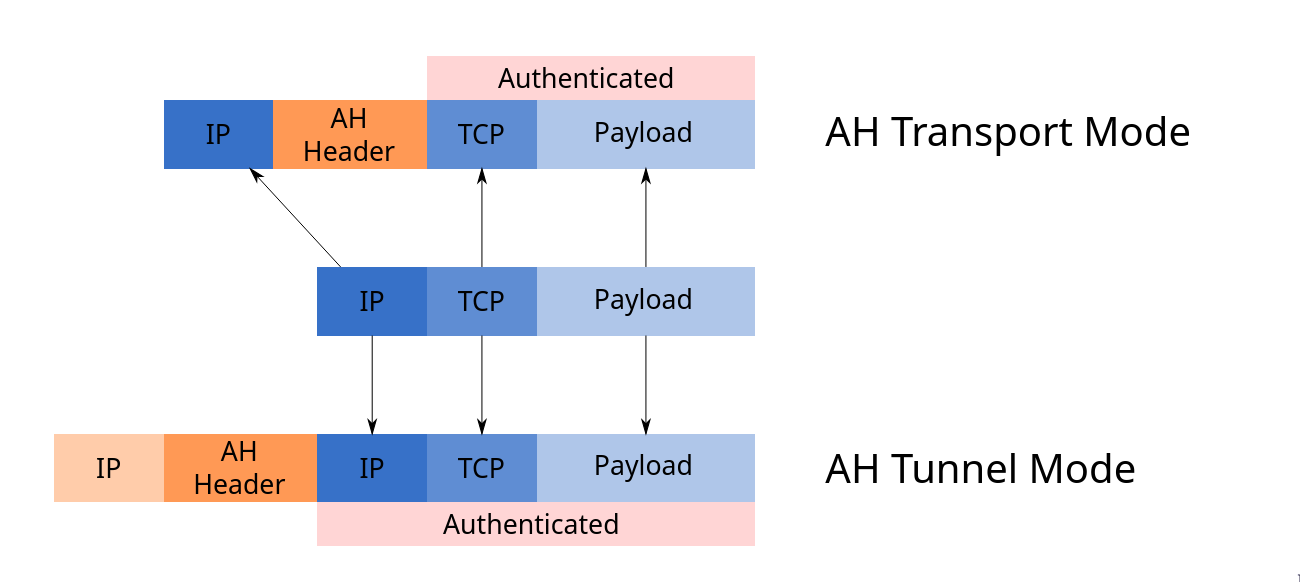
\includegraphics[width=0.6\linewidth]{images/ah_transport_tunnel.png}\\
    {\small (a) AH — Transport / Tunnel}
    \vspace{0.6cm}

    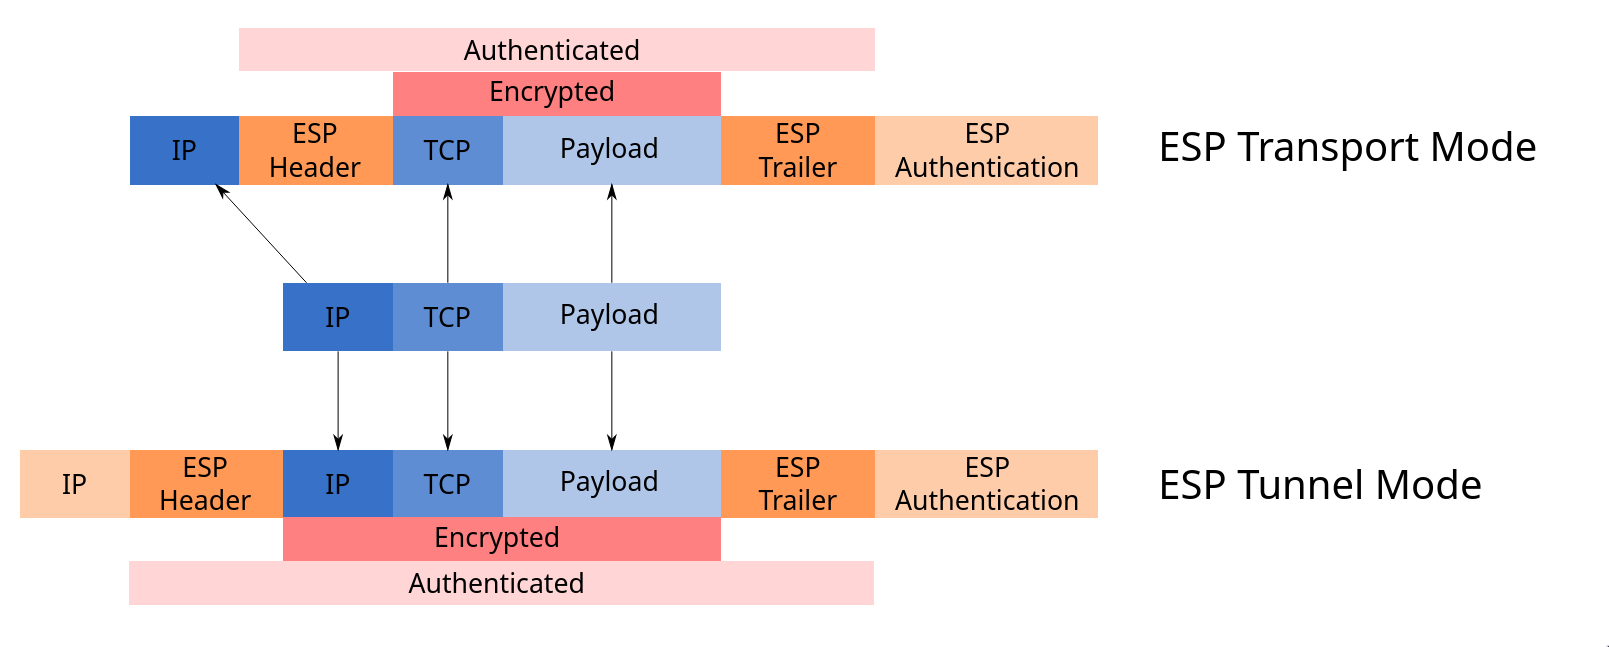
\includegraphics[width=0.6\linewidth]{images/esp_transport_tunnel.png}\\
    {\small (b) ESP — Transport / Tunnel}
    \caption{Confronto: AH e ESP nelle modalità Transport e Tunnel.}
    \label{fig:ah_esp_transport_tunnel}
\end{figure}

\subsubsection{Traffic Flow Confidentiality (TFC)}

Sebbene la cifratura ESP garantisca che il contenuto e il campo \textit{Next Header} siano illeggibili — impedendo a un osservatore di distinguere deterministicamente il protocollo applicativo (es. VoIP vs SMTP) — la sola cifratura non garantisce la \textbf{unlinkability} (non collegabilità).
Come evidenziato dagli studi su \textit{Statistical Traffic Pattern Analysis}, rimangono esposti metadati critici come la dimensione dei pacchetti e la temporizzazione degli invii.

\textbf{NOTA:} L'attacco si chiama \textit{Statistical Traffic Analisys} mentre il metodo di difesa prende il nome di \textit{Traffic Flow Confidentiality}.

\paragraph{La Minaccia: Traffic Fingerprinting}
Anche in un tunnel cifrato, servizi diversi generano "forme" di traffico diverse. Ad esempio, visitare \texttt{amazon.com} genera un profilo statistico di dimensioni dei pacchetti molto diverso da quello di un video su YouTube. Un attaccante può utilizzare queste "impronte" (\textit{fingerprinting}) per dedurre quale sito o servizio l'utente sta utilizzando, pur non potendo leggere i dati.
Per mitigare questa minaccia si possono agire su tre leve principali: la dimensione dei pacchetti, la temporizzazione degli invii e la presenza/assenza di pacchetti. IPsec fornisce supporto soltanto parziale alla prima leva (mascheramento delle dimensioni).

Per contrastare queste analisi, ESP implementa due specifiche contromisure di \textit{Traffic Flow Confidentiality}:

\begin{enumerate}
    \item \textbf{Mascheramento della Dimensione (TFC Padding)}:
    Il padding standard di ESP (necessario per l'allineamento ai blocchi dell'algoritmo di cifratura, es. AES-CBC) è limitato a 255 byte, spesso insufficienti per nascondere la reale natura del payload.
    ESP introduce quindi un \textbf{TFC Padding} supplementare: permette di aggiungere dati riempitivi arbitrari per alterare la dimensione del pacchetto.
    \begin{itemize}
        \item Questo consente di rendere tutti i pacchetti di dimensione uniforme (o casuale), nascondendo la lunghezza reale del messaggio originale.
    \end{itemize}

    \item \textbf{Mascheramento della Frequenza (Dummy Packets)}:
    Per nascondere i momenti di silenzio o la frequenza di trasmissione (che distinguerebbe un traffico \textit{Variable Bit Rate} - VBR, come la navigazione web, da uno costante), ESP può generare traffico fittizio.
    \begin{itemize}
        \item Vengono inviati pacchetti "vuoti" con il campo \textbf{Next Header impostato a 59} (valore riservato per "No Next Header").
        \item Il ricevente, decifrato il pacchetto e letto il Next Header 59, scarta immediatamente il pacchetto trattandolo come "dummy".
    \end{itemize}
\end{enumerate}

\begin{figure}[ht!]
    \centering
    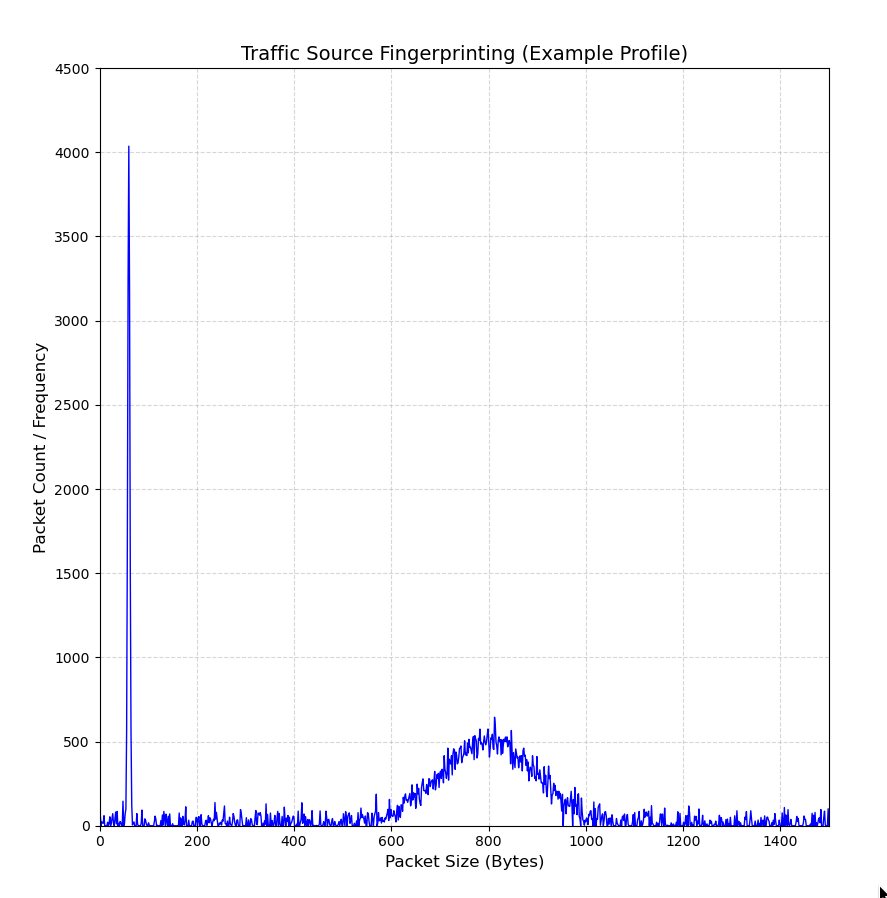
\includegraphics[width=0.40\linewidth]{images/fingerprint.png}
    \caption{Esempio di "impronta" di un sito}
    \label{fig:fingerprint}
\end{figure}

\section{IKEv2}

Per stabilire e mantenere in modo scalabile le Security Associations (SA) si utilizza IKE (Internet Key Exchange); la versione corrente è IKEv2 (RFC 7296). IKEv2 automatizza la negoziazione dei parametri di protezione (AH/ESP, modalità, algoritmi), la derivazione e il rinnovo delle chiavi e la selezione delle policy di traffico, risolvendos i limiti della gestione manuale (manual keying) e garantendo proprietà moderne come il rekeying e la Perfect Forward Secrecy.

Concettualmente IKEv2 distingue due tipologie di SA: l'IKE SA, che protegge gli stessi messaggi di controllo di IKE, e le CHILD SA, che proteggono il traffico dati (ESP o AH). Lo scambio tipico si articola in una prima fase di negoziazione dei parametri crittografici e di Diffie-Hellman (\texttt{IKE\_SA\_INIT}), seguita dall'autenticazione dei peer e dalla creazione della prima CHILD SA (\texttt{IKE\_AUTH}).
Successivamente si possono creare ulteriori CHILD SA tramite \texttt{CREATE\_CHILD\_SA} e gestire notifiche o chiusure con messaggi INFORMATIONAL.

\begin{description}
    \item [IKE SA:] È una Security Association utilizzata per scambiare i messaggi di controllo del protocollo IKE stesso.
    \item [CHILD SA:] È una Security Association utilizzata per scambiare i messaggi di dati veri e propri, utilizzando i protocolli AH o ESP. Possono essere stabilite molteplici CHILD SA tra due peer.
\end{description}

\begin{figure}[ht!]
    \centering
    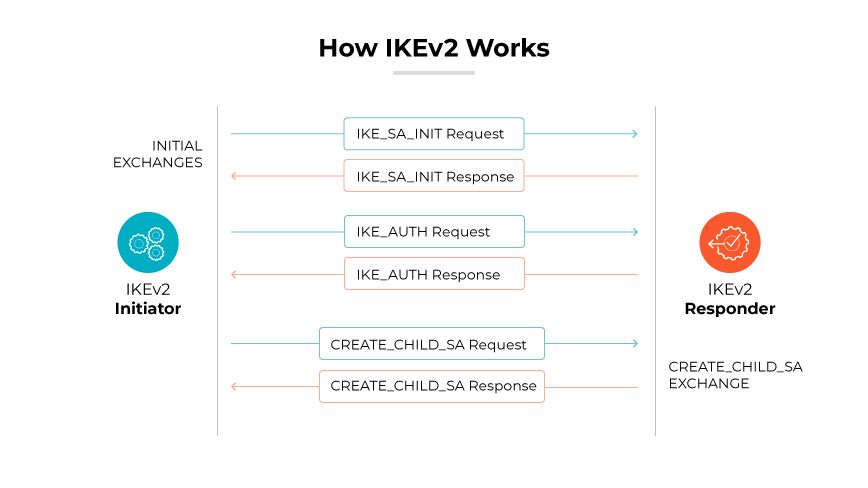
\includegraphics[width=0.7\linewidth]{images/ike_1.png}
    \caption{Messaggi IKEv2}
    \label{fig:ike}
\end{figure}

Operativamente, IKEv2 gira su UDP (porta 500, o 4500 quando è attivo il NAT-Traversal) e include meccanismi integrati di ritrasmissione e riconoscimento per garantire affidabilità. Un messaggio IKE è incapsulato sopra UDP e contiene un header seguito da una sequenza di payload tipizzati:
\[
    [\text{IP}] [\text{UDP}] [\text{IKE header}] [\text{Payload}_1] \ldots [\text{Payload}_N]
\]
I payload sono concatenati e ogni payload possiede un piccolo header con campo \texttt{Next Payload}, un bit \texttt{Critical} (che, se impostato, obbliga il destinatario a rifiutare il messaggio se non supporta quel payload) e la lunghezza del payload. Questa struttura a catena rende IKEv2 estendibile: nuovi tipi di payload possono essere aggiunti senza rompere la compatibilità verso implementazioni più vecchie.

L'header IKE contiene, fra gli altri, gli identificatori Initiator SPI e Responder SPI (8 byte ciascuno), il Message ID per correlare richieste/risposte e gestire ritrasmissioni/replay, il tipo di exchange (es. \texttt{IKE\_SA\_INIT}, \texttt{IKE\_AUTH}, \texttt{CREATE\_CHILD\_SA}) e la lunghezza totale del messaggio. Questi elementi permettono a IKEv2 di correlare le sequenze di messaggi, supportare ritrasmissioni e prevenire replay, mantenendo al contempo flessibilità e sicurezza nella negoziazione delle SA.

\begin{figure}[ht!]
    \centering
    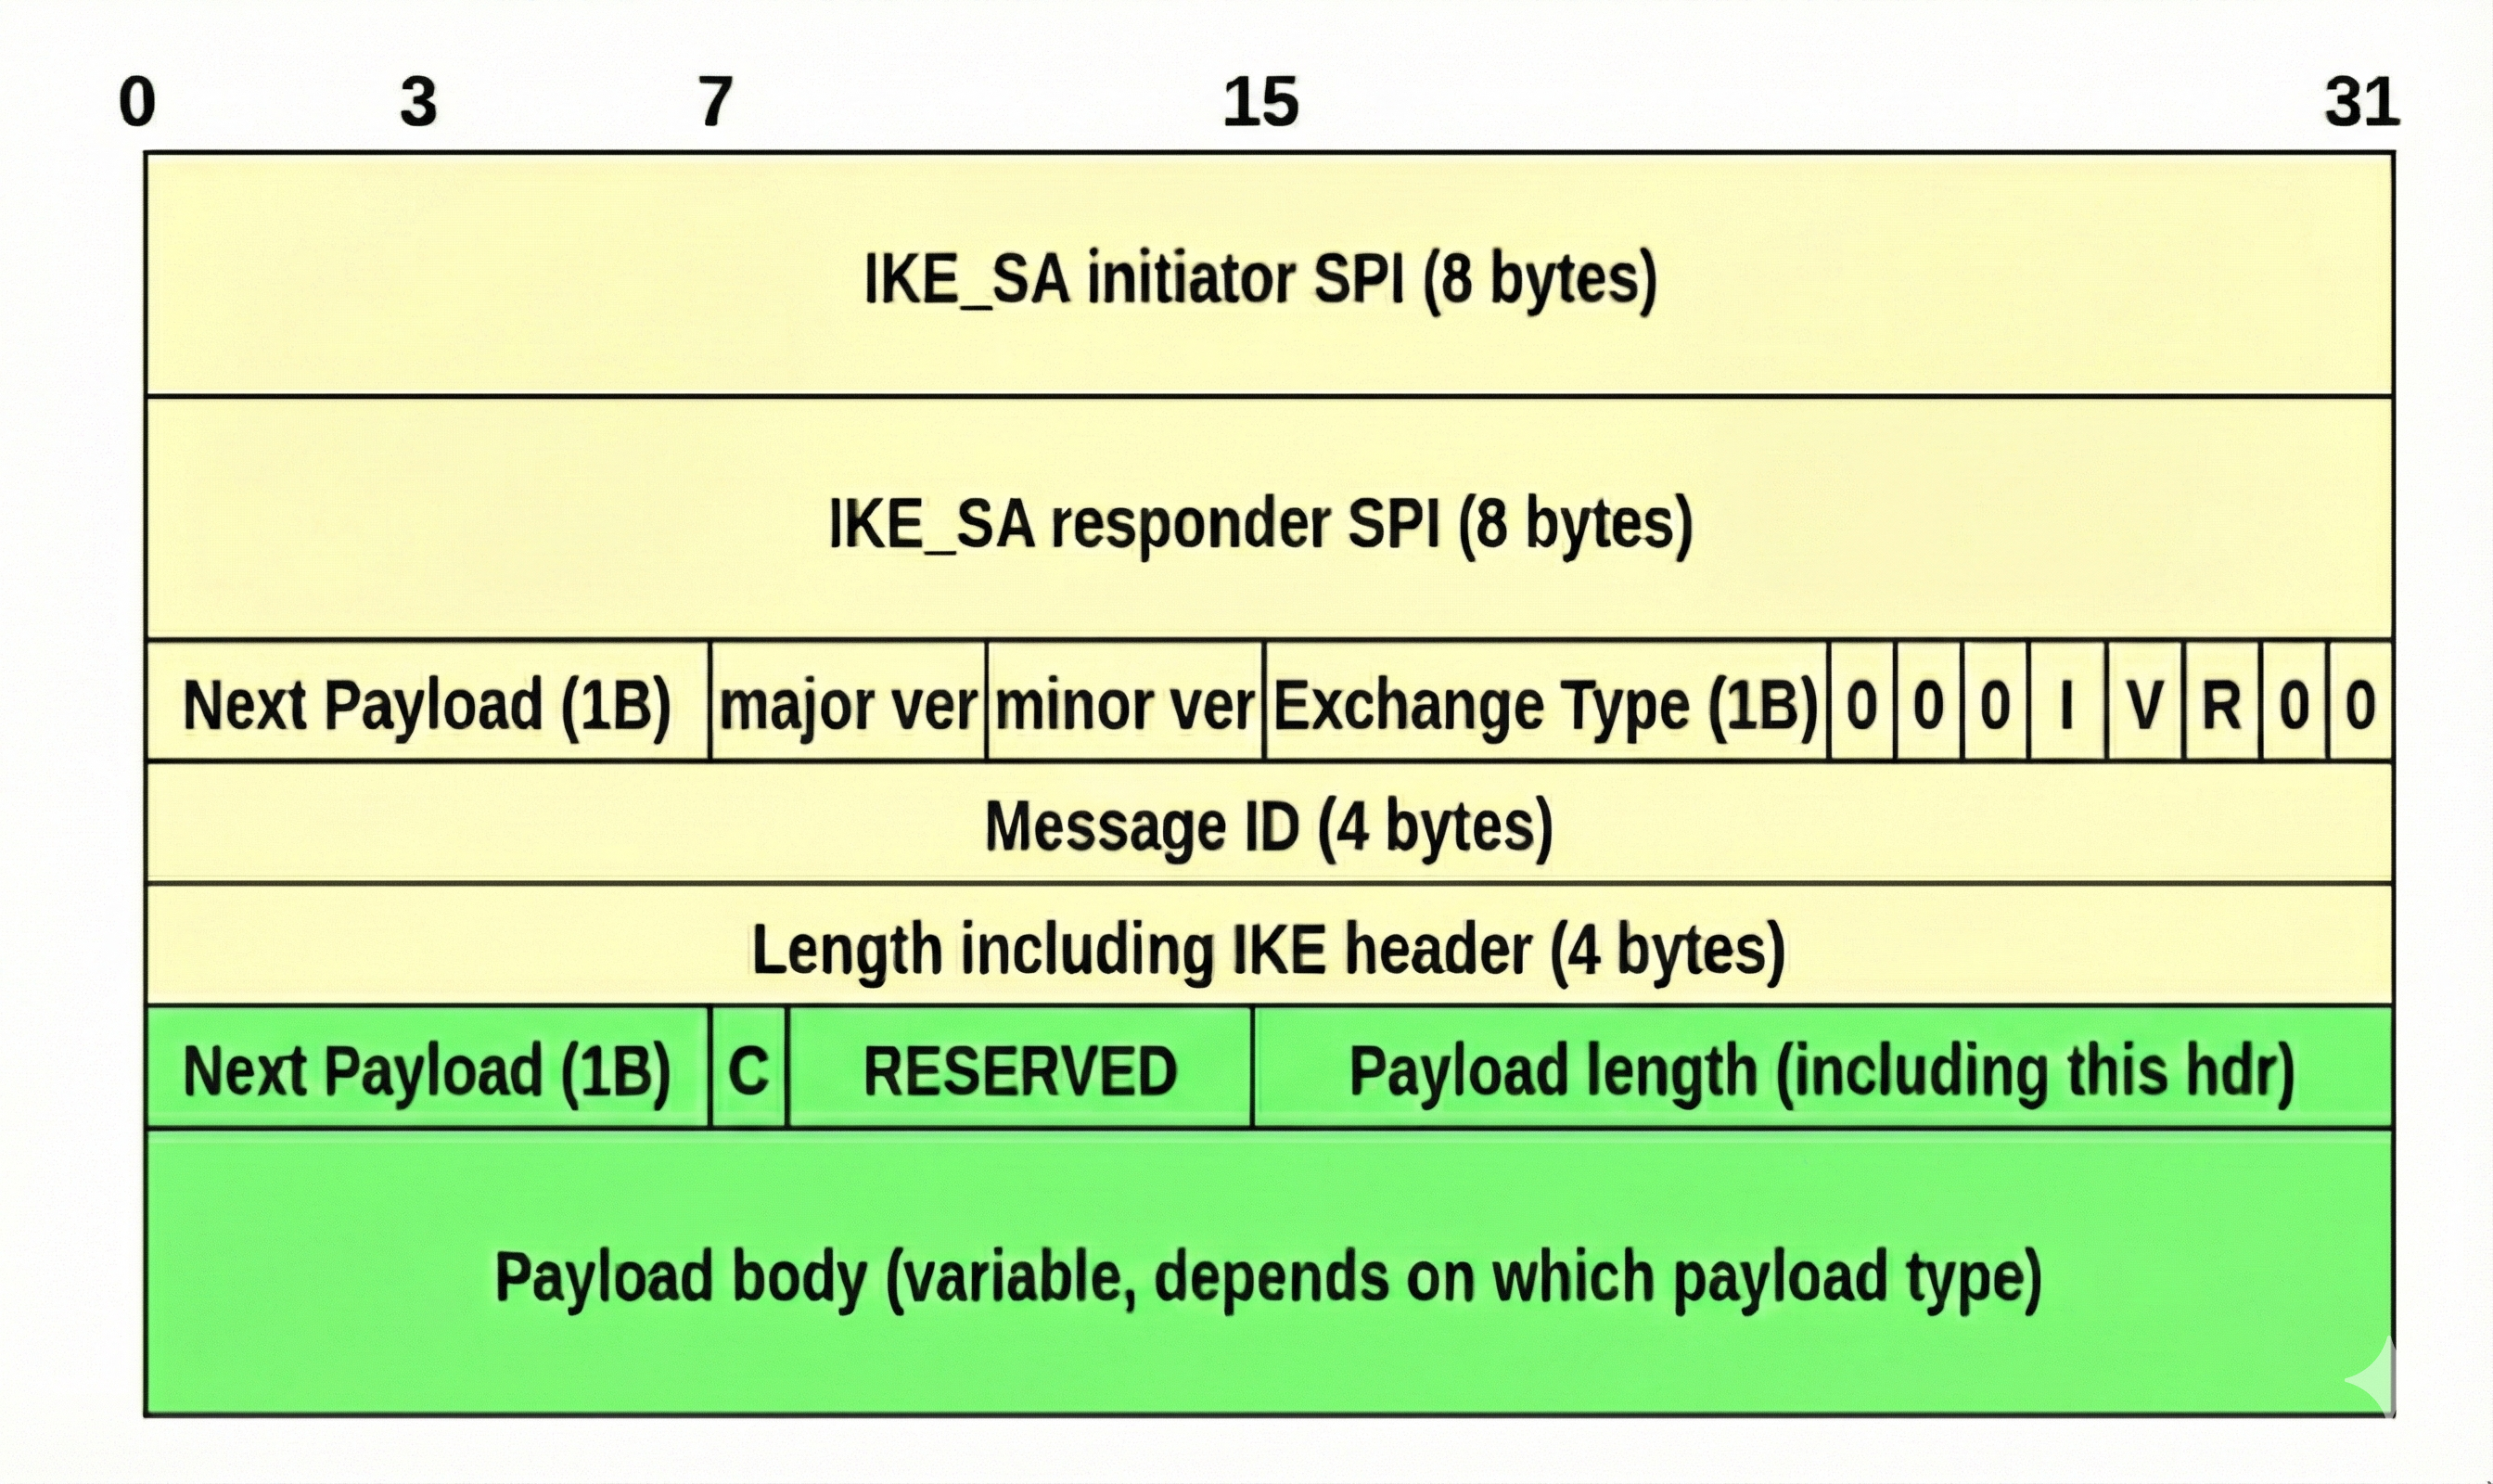
\includegraphics[width=0.7\linewidth]{images/ike_2.png}
    \caption{Header IKEv2}
    \label{fig:ike_header}
\end{figure}

Il bit o flag V sta per "Version".
\begin{description}
    \item[V = 0:] "Questa è la mia versione massima" oppure "Non sto segnalando capacità superiori".
    \item[V = 1:] "Sto usando questa versione (es. N-1) per compatibilità, ma in realtà sono capace di parlare una versione più recente (es. N)".
\end{description}

\subsection{Handshake regolare e attacco Man-in-the-Middle}

\begin{figure}[ht!]
    \centering
    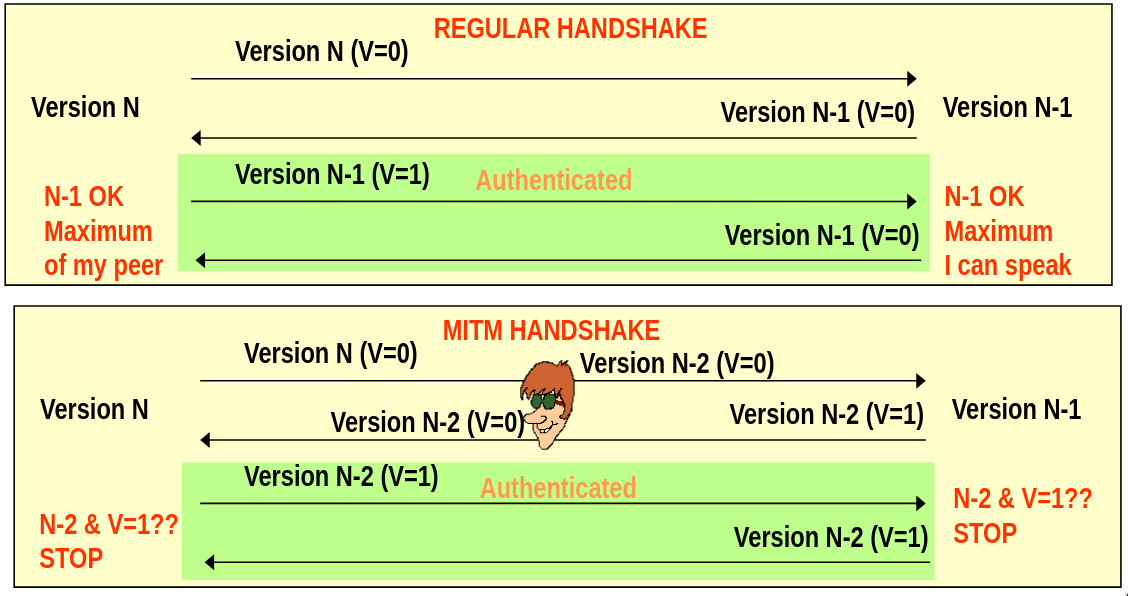
\includegraphics[width=0.7\linewidth]{images/ike_3.png}
    \caption{Utilizzo bit $V$}
    \label{fig:ike_vbit}
\end{figure}

\begin{description}
    \item[Handshake regolare]
    Consideriamo prima il caso ideale senza attaccanti. L'Initiator supporta la versione \texttt{N}, il Responder la versione \texttt{N-1}. L'Initiator propone \texttt{N} e il Responder risponde che al massimo può arrivare a \texttt{N-1}. Dopo la fase di negoziazione iniziale, quando la comunicazione è ormai cifrata e autenticata, l'Initiator invia messaggi usando la versione concordata (\texttt{N-1}) ma segnala con il flag \texttt{V=1} che lui sarebbe comunque in grado di usare una versione più recente (\texttt{N}). Il Responder, vedendo questa informazione autenticata, conclude correttamente che la scelta comune è \texttt{N-1} e la connessione procede normalmente.
    \item[Handshake sotto attacco MITM.]
    Nello scenario con un attaccante che opera in mezzo, l'obiettivo dell'avversario è forzare entrambe le parti a scendere a una versione molto vecchia e vulnerabile (\texttt{N-2}). L'Initiator invia la proposta \texttt{N}, ma l'attaccante altera il pacchetto in transito trasformandolo in \texttt{N-2}. Il Responder, credendo che l'altro sia antiquato, accetta \texttt{N-2} ma imposta il flag \texttt{V=1} per indicare autenticata capacità di usare \texttt{N-1}. L'attaccante però rimuove o azzera questo flag prima di inoltrare la risposta all'Initiator, nascondendo così al mittente la reale capacità del Responder. A questo punto parte la fase autenticata: l'Initiator, convinto di parlare con \texttt{N-2}, invia messaggi autenticati che includono il flag \texttt{V=1} (segno che lui supporta \texttt{N}). Il Responder riceve ora, all'interno della parte autenticata, un messaggio che dichiara \texttt{V=1} mentre la negoziazione iniziale in chiaro aveva stabilito \texttt{N-2}. Questo conflitto è un chiaro indicatore di manomissione della negoziazione in chiaro, perché implica che qualcuno ha modificato i messaggi prima dell'instaurazione della protezione. Di conseguenza il Responder rifiuta la connessione e l'handshake viene interrotto, impedendo il downgrade forzato.
\end{description}

Questo meccanismo intelligente (il flag V) non esiste in IKEv1. Quindi, se un attaccante riesce a forzare un downgrade fino alla versione 1 del protocollo, questo controllo di sicurezza non scatta e l'attacco ha successo. Ecco perché disabilitare IKEv1 sui server moderni è fondamentale.

\subsection{FASE 1: Exchange Info - \texttt{IKE\_SA\_INIT}}

In questa prima fase i due peer si scambiano le informazioni iniziali necessarie per concordare "come" proteggeranno le comunicazioni successive. I messaggi viaggiano in chiaro e contengono le proposte di parametri (algoritmi di crittografia, integrità, PRF e gruppi Diffie-Hellman), i valori effimeri per il key exchange e i nonce casuali: tutto ciò serve a costruire una base crittografica condivisa ma non ancora autenticata. 

Lo scopo pratico è duplice: da un lato selezionare in modo interoperabile le primitive crittografiche che verranno poi usate; dall'altro raccogliere il materiale  necessario per eseguire il Diffie-Hellman e ottenere una secret root comune. Poiché questa negoziazione è in chiaro, le informazioni trasmesse devono essere tali da non compromettere le proprietà essenziali (le chiavi finali sono comunque protette dalle proprietà del DH e dai nonce).

Come risultato di \texttt{IKE\_SA\_INIT} si ottiene SKEYSEED, una chiave di partenza calcolata tramite la PRF negoziata sui valori DH e sui nonce; da SKEYSEED verranno poi derivate tutte le chiavi operative (autenticazione, cifratura e materiale per le CHILD SA). Questa fase costituisce quindi il fondamento crittografico su cui si appoggiano le successive fasi di autenticazione e creazione delle SA dati.

\paragraph{Payload scambiati}
\begin{itemize}
    \item \textbf{SAi1 / SAr1 (Security Association)}: l'Initiator propone la lista degli algoritmi supportati; il Responder seleziona le proposte accettate per funzione (crittografia, integrità/PRF, DH).
    \item \textbf{KEi / KEr (Key Exchange)}: valori effimeri per lo scambio Diffie-Hellman.
    \item \textbf{Ni / Nr (Nonce)}: numeri casuali (minimo 16 byte) usati per la derivazione delle chiavi e per prevenire replay.
    \item \textbf{CERTREQ (opzionale)}: richiesta di certificati.
\end{itemize}

\begin{tcolorbox}[colback=blue!5,colframe=blue!40!black,title=Nota]
Diversamente da TLS, dove le cipher suite sono spesso fornite come combinazioni predefinite, in IKEv2 è possibile negoziare separatamente le primitive crittografiche (cifratura, autenticazione, PRF, gruppo DH), consentendo di ottenere liberamente qualsiasi combinazione di algoritmi.
\end{tcolorbox}

\paragraph{Calcolo delle chiavi}
Al termine di \texttt{IKE\_SA\_INIT} viene calcolata la secret root:
\[
    \mathrm{SKEYSEED} = \mathrm{prf}(N_i,\; N_r,\; g^{ir})
\]
dove \(\mathrm{prf}\) è la funzione pseudo-casuale negoziata durante l'handshake e $g^{ir}$ è il DH coefficient.

A partire da SKEYSEED si deriva un insieme di chiavi tramite una costruzione estesa della PRF (spesso indicata come \(\mathrm{prf+}\)), utilizzando inoltre i Nonce e gli SPI:

\begin{itemize}
    \item \(\mathrm{SK}_{ai},\ \mathrm{SK}_{ar}\): chiavi di autenticazione (Initiator / Responder).
    \item \(\mathrm{SK}_{ei},\ \mathrm{SK}_{er}\): chiavi di cifratura.
    \item \(\mathrm{SK}_{pi},\ \mathrm{SK}_{pr}\): chiavi usate per generare il payload AUTH nella fase successiva.
    \item \(\mathrm{SK}_{d}\): materiale chiave fondamentale per derivare le chiavi delle future CHILD\_SA (traffic SA).
\end{itemize}

Nota: a differenza di TLS, la PRF in IKEv2 è negoziabile; ciò permette di scegliere la funzione di derivazione più adatta durante la negoziazione.

\subsubsection{Protezione dagli attacchi DoS (Denial of Service)}

Gli scambi iniziali di IKEv2 richiedono operazioni costose (calcoli Diffie-Hellman, allocazione di strutture di stato, derivazione di chiavi). Un avversario può sfruttare questo fatto inviando molteplici richieste iniziali forgiate (spesso con IP sorgente spoofato) per costringere il Responder a consumare CPU e memoria e quindi degradare o interrompere il servizio. 

Per mitigare questo rischio IKEv2 adotta un meccanismo di \textbf{stateless cookie handshake} (handshake a 4 vie) che consente al Responder di verificare l'autenticità della richiesta senza allocare immediatamente stato persistente. Di seguito una descrizione dettagliata e robusta del meccanismo.

\paragraph{Obiettivo}
Ridurre il costo computazionale e la memoria usata dal Responder in risposta a richieste iniziali non verificate, obbligando il peer legittimo a dimostrare la raggiungibilità dell'indirizzo IP sorgente prima che il Responder esegua operazioni pesanti.

\paragraph{Sequenza di messaggi (4-way stateless cookie)}
\begin{enumerate}
    \item \textbf{INIT (da Initiator a Responder)}: l'Initiator invia SAi1 | KEi | Ni (proposta SA, valore DH effimero, nonce).
    \item \textbf{COOKIE-REPLY (da Responder a Initiator)}: il Responder risponde \emph{senza} allocare stato e \emph{senza} eseguire DH, inviando un messaggio contenente solo un cookie e il proprio Ni o una indicazione di richiesta cookie.
    \item \textbf{INIT+COOKIE (da Initiator a Responder)}: l'Initiator ritrasmette la proposta originaria includendo il cookie ricevuto.
    \item \textbf{Verifica e continuazione (da Responder)}: il Responder verifica il cookie. Se valido, allora alloca lo stato (SPI) ed esegue le operazioni DH/derive necessarie e prosegue con il normale IKE\_SA\_INIT/ IKE\_AUTH.
\end{enumerate}

Il cookie non deve essere né statico (ad esempio rigenerato ogni 10 minuti), perché in quel caso un avversario potrebbe inviare un \texttt{IKE\_SA\_INIT} e poi riutilizzare il cookie senza attendere la richiesta legittima dal server. Allo stesso modo non può essere completamente casuale, poiché ciò implicherebbe la necessità di memorizzarlo sul Responder per poterlo verificare. Pertanto il cookie dovrebbe essere derivato in modo deterministico da parametri crittografici della richiesta (es. nonce, SPI, eventuali campi stabili dell'IP/porta), permettendo la verifica senza mantenere stato persistente.

\paragraph{Proprietà desiderate del Cookie}
\begin{itemize}
    \item \textbf{Statelessness del Responder}: il Responder non deve mantenere una tabella di cookie emessi (evita consumo di memoria e race condition).
    \item \textbf{Unicità e legame alla richiesta}: il cookie deve legarsi in modo affidabile ai parametri della richiesta (es. nonce, IP/port, SPI) così che solo chi possiede il controllo dell'indirizzo IP sorgente possa riproporre la richiesta con il cookie valido.
    \item \textbf{Resistenza alla predizione e riproduzione}: il cookie deve essere calcolato con una funzione crittografica sicura e un segreto noto solo al Responder; il segreto deve ruotare periodicamente per limitare la finestra di validità dei cookie.
\end{itemize}

\paragraph{Esempio di costruzione del Cookie}
Un costrutto sicuro e pratico è l'uso di una MAC o HMAC:
\[
    \text{Cookie} \;=\; \text{VersionID} \,\|\, \text{HMAC}_{K_{\text{secret}}}\big(\,N_i \,\|\; \text{IP}_i \,\|\; \text{Port}_i \,\|\; \text{SPI}_i \,\big)
\]
dove
\begin{itemize}
    \item \(N_i\) = nonce dell'Initiator,
    \item \(\text{IP}_i,\ \text{Port}_i\) = indirizzo e porta sorgente (attenzione a NAT; vedere nota),
    \item \(\text{SPI}_i\) = SPI proposto dall'Initiator,
    \item \(K_{\text{secret}}\) = segreto periodicamente rinnovato dal Responder
\end{itemize}

Il campo VersionID permette di gestire formati diversi di cookie durante aggiornamenti del protocollo.

\paragraph{Validazione e politiche operative}
\begin{description}
    \item[Ricezione] 
    Il Responder riceve il messaggio \texttt{IKE\_SA\_INIT} riformulato dall'Initiator, il quale ora include il Cookie che era stato precedentemente generato e inviato dal Responder stesso.

    \item[Ricalcolo] 
    Il Responder ricalcola il valore HMAC sui dati contenuti nella richiesta (ad esempio SPI, Nonce, IP) utilizzando il proprio segreto locale ($K_{\text{secret}}$). Per evitare fallimenti durante la rotazione delle chiavi, il Responder verifica la validità del cookie anche utilizzando il segreto immediatamente precedente.

    \item[Confronto e Allocazione] 
    Il Responder confronta l'HMAC appena calcolato con il valore del Cookie presente nel pacchetto ricevuto:
    \begin{itemize}
        \item \textbf{Verifica superata:} Se i valori corrispondono, l'indirizzo IP dell'Initiator è confermato. Solo in questo momento il Responder \textbf{alloca lo stato} in memoria e procede con la negoziazione.
        \item \textbf{Verifica fallita:} Se i valori non corrispondono, il pacchetto viene ignorato e non viene allocata alcuna risorsa (nessuno stato viene memorizzato).
    \end{itemize}
\end{description}

\subsection{FASE 2: \texttt{IKE\_AUTH}}

La fase \texttt{IKE\_AUTH} segue immediatamente lo scambio iniziale (\texttt{IKE\_SA\_INIT}). A differenza della fase precedente, tutti i payload scambiati in questa fase sono \textbf{crittografati e autenticati} (ad eccezione dell'header IKE).

Gli obiettivi principali di questa fase sono autenticare le identità dei peer, verificare l'integrità dello scambio precedente e stabilire la prima connessione dati (CHILD\_SA).

\begin{itemize}
    \item \textbf{Protezione del Messaggio:} Il messaggio viene cifrato utilizzando la chiave di cifratura ($SK_e$) e autenticato con la chiave di autenticazione ($SK_a$), entrambe derivate durante la fase INIT.
    \item \textbf{Algoritmi:} Vengono utilizzati gli algoritmi di crittografia e autenticazione negoziati precedentemente.
\end{itemize}

Lo scambio prevede l'invio di diversi payload critici:

\begin{itemize}
    \item \textbf{IDi / IDr (Identities):} Identificativi dell'Initiator e del Responder. Possono essere indirizzi IP, nomi di dominio (FQDN), indirizzi email o altro.
    \item \textbf{CERT / CERTREQ:} Payload opzionali per l'invio di certificati digitali o la richiesta di certificati al peer.
\end{itemize}

\subsubsection{Il Payload AUTH}
Questo è il componente fondamentale per la sicurezza dello scambio:
\begin{itemize}
    \item \textbf{Funzione:} Autentica il messaggio precedente (INIT) e le identità dichiarate ($ID_i, ID_r$).
    \item \textbf{Prevenzione Attacchi:} Firmando crittograficamente i messaggi precedenti, questo payload combatte efficacemente i \textit{downgrade attacks} (impedendo a un attaccante di modificare la negoziazione in chiaro della fase INIT).
    \item \textbf{Metodo:} Se si utilizzano certificati, l'autenticazione avviene tramite la corrispondente chiave privata.
\end{itemize}

\subsection{Generazione della CHILD\_SA}
Durante la fase \texttt{IKE\_AUTH} viene creata anche la prima \texttt{CHILD\_SA} (il tunnel per il traffico dati vero e proprio).

\begin{itemize}
    \item \textbf{Incorporazione:} La negoziazione della prima SA figlia è direttamente incorporata nei messaggi AUTH, evitando round-trip aggiuntivi.
    \item \textbf{Nuovi Parametri:} Vengono trasmessi i payload $SA$ ($SA_{i2}, SA_{r2}$) per negoziare i parametri di sicurezza specifici per questa connessione dati.
    \item \textbf{Traffic Selectors (TS):} Vengono definiti i parametri $TS_i$ e $TS_r$ che specificano quale traffico deve passare nel tunnel.
    \begin{itemize}
        \item Includono intervalli di indirizzi IP (es. 192.168.1.1-12), numeri di porta e protocolli.
        \item Questi parametri vengono confrontati con la Security Policy Database (SPD) locale.
    \end{itemize}
\end{itemize}

\begin{tcolorbox}[colback=blue!5,colframe=blue!40!black,title=PER L'ESAME]
Il prof ha esplicitamento detto che gli interessa maggiormente come avviene l'attacco MITM alla versione e come proteggerci, il cookie e come funziona \texttt{IKE\_SA\_INIT}.
\end{tcolorbox}
\end{document}